\documentclass[12pt]{article}
\usepackage[spanish]{babel}
\usepackage[utf8]{inputenc}
\usepackage{csquotes}

% Interlineado 1.5
\usepackage{setspace}
\onehalfspacing

% Fuente Times New Roman
\usepackage{mathptmx}

% Acomodar margenes del documento
\usepackage[a4paper, margin=2cm, top=3cm, headheight=50pt]{geometry}

% Paquetes comunes
\usepackage{graphicx, float}
\usepackage{amsfonts, amssymb, amsmath}
\usepackage{physics, esvect}
\usepackage{enumerate}
\usepackage[colorlinks=true, citecolor=blue]{hyperref}

% Nuevos
\usepackage{pgfplots}
\usepackage{tikz, color}
\usepackage{tikz-3dplot}
\pgfplotsset{width=15cm, compat=1.18}
\usepgfplotslibrary{fillbetween}
\usepgfplotslibrary{external}
\tikzexternalize[prefix=figs/]


% Encabezados
\usepackage{fancyhdr}
\pagestyle{fancy}
\fancyhf{}
\fancyfoot[C]{\thepage}
\fancyhead[L]{
  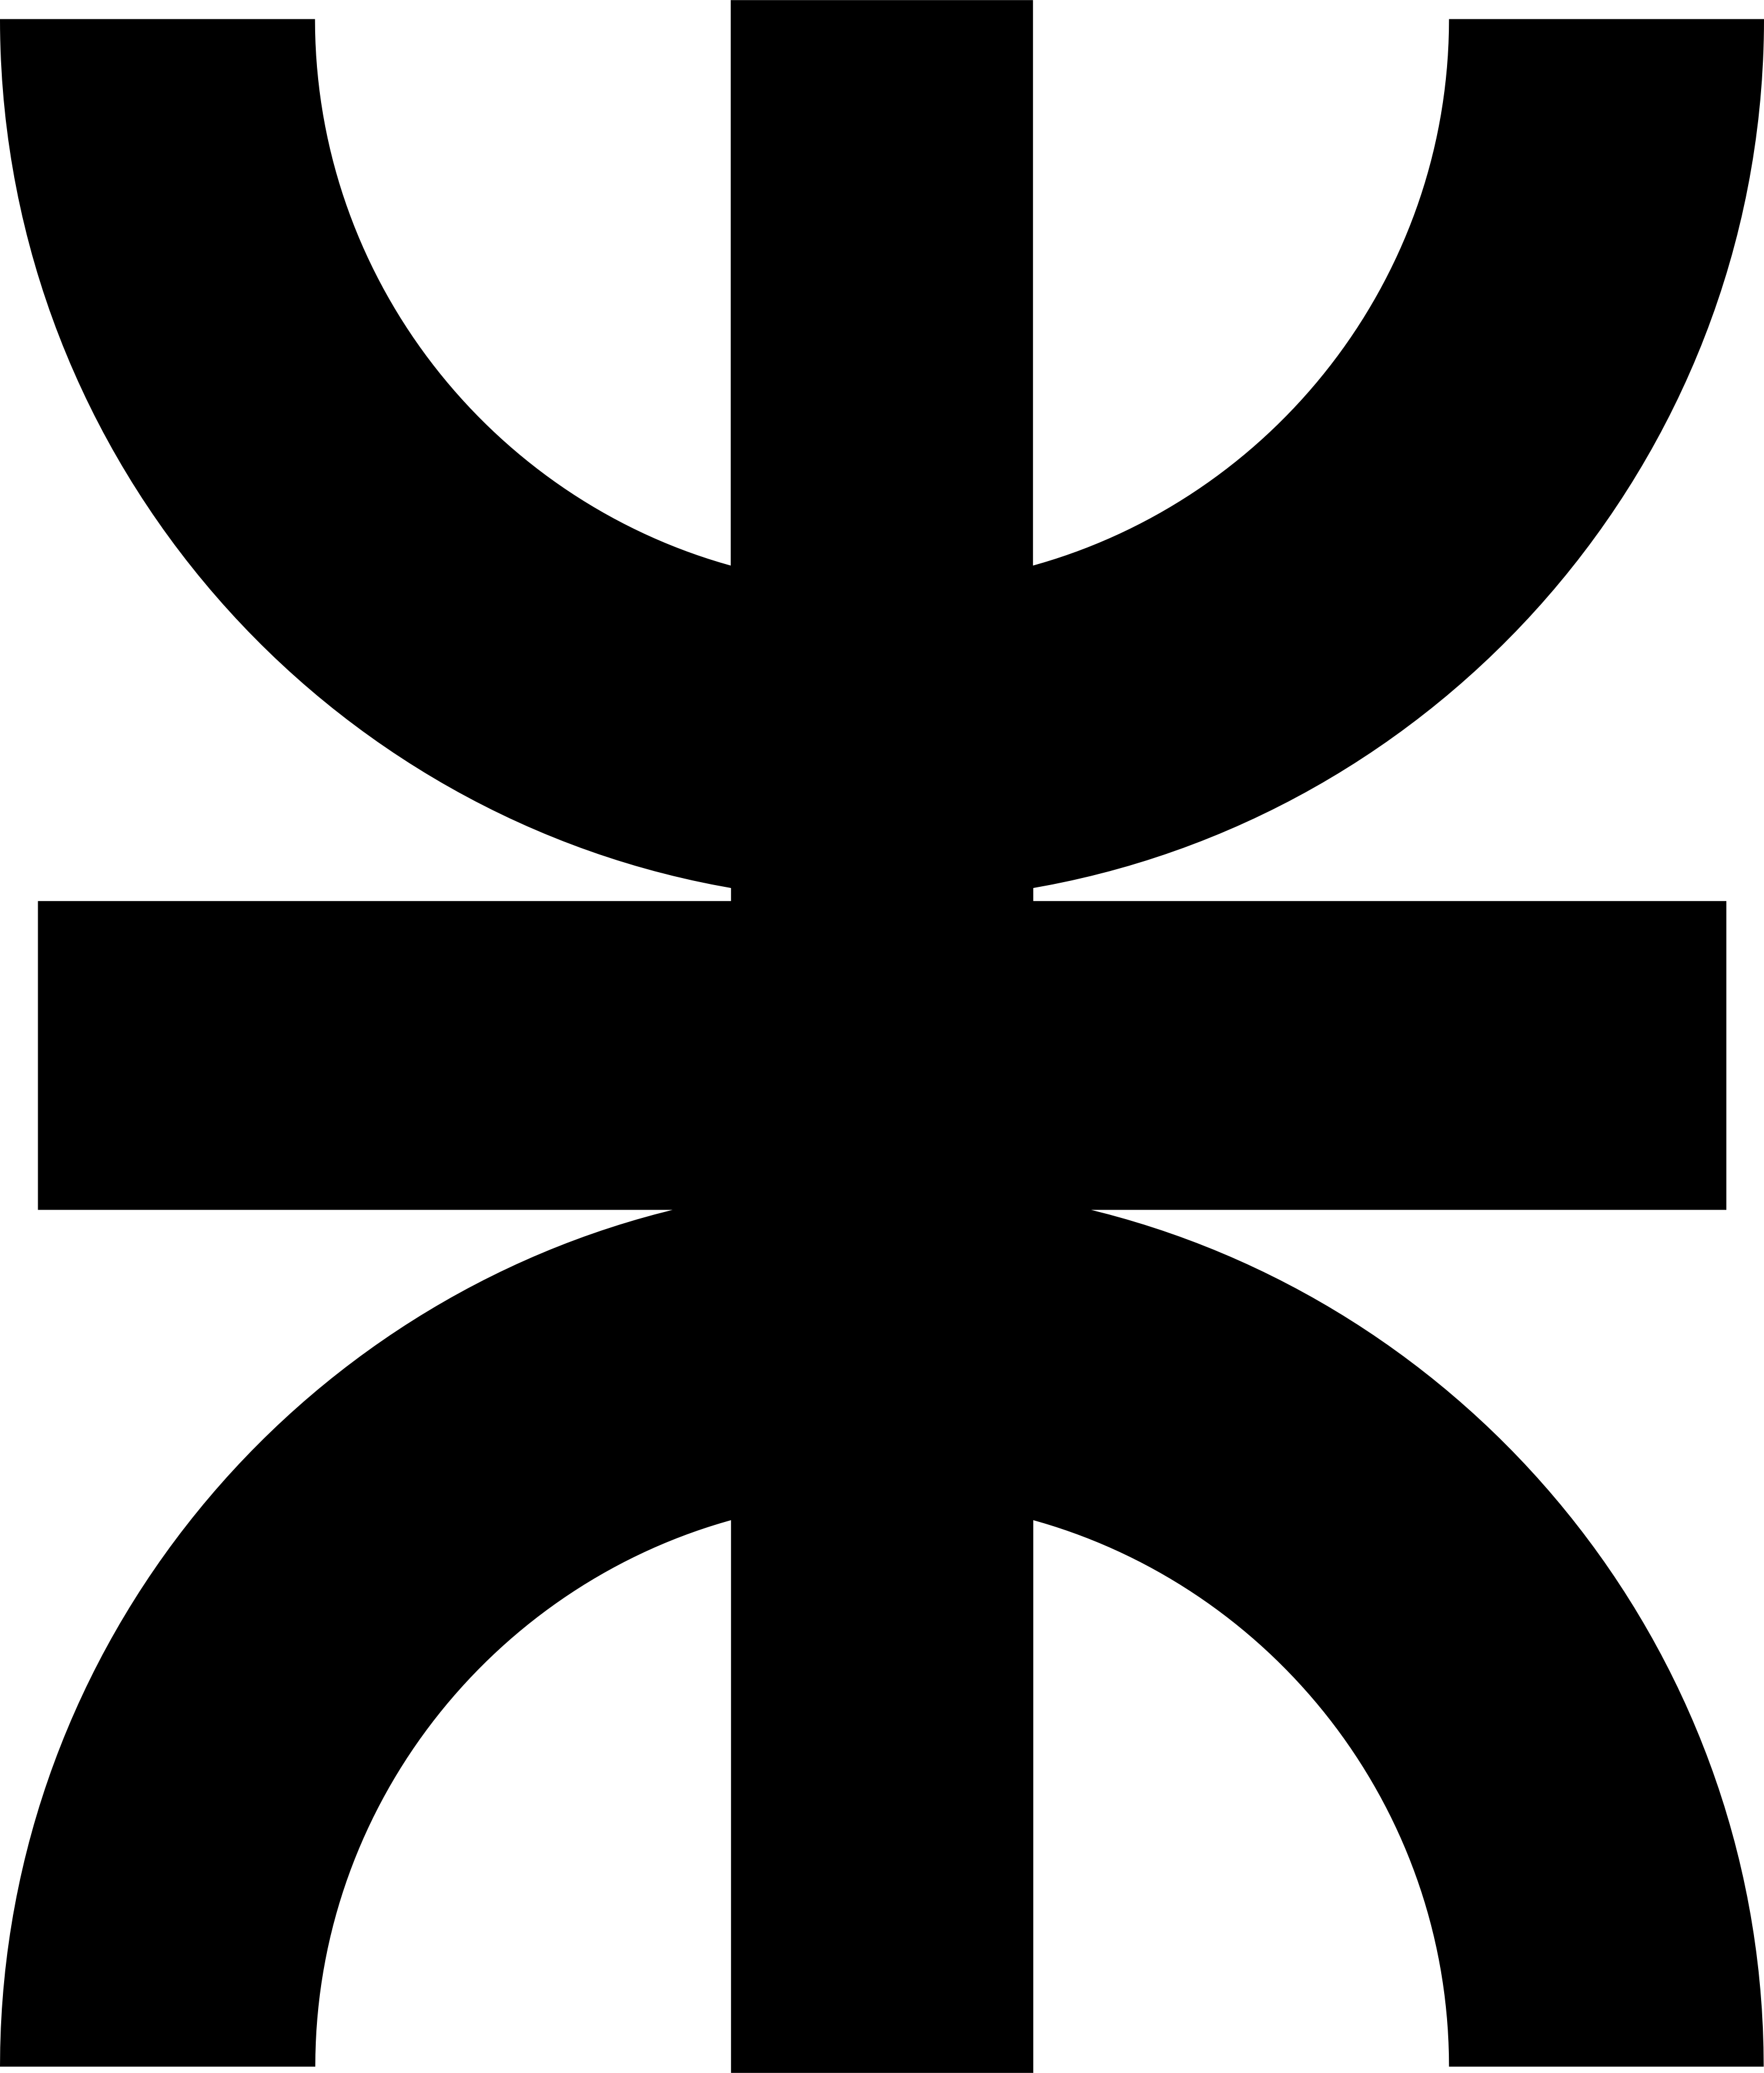
\includegraphics[height=1.2cm]{~/imagenes/logo_utn.png}
  \shortstack[l]{
    {\footnotesize Universidad Tecnológica Nacional} \\
    {\footnotesize Facultad Regional Córdoba} \\
    {\footnotesize Extensión Áulica Bariloche}
  }
}
\fancyhead[C]{
  \shortstack[c]{
    {\footnotesize Análisis Matemático 2} \\
    {\footnotesize Resumen} \\
    {\footnotesize }
  }
}
\fancyhead[R]{
  \shortstack[r]{
    {\footnotesize Profesor: Mónica Guraya} \\
    {\footnotesize Alumno: Ricardo Nicolás Freccero} \\
    {\footnotesize Fecha: 19/04/2025}
  }
}

% Para bibliografía
\usepackage[backend=biber, style=apa]{biblatex}
\addbibresource{bibliografia.bib}

\begin{document}
\newgeometry{margin=2cm, top=1.5cm}
\begin{titlepage}
	\centering
	
\includegraphics[width=\linewidth]{~/imagenes/logo_utn_frc.jpg}\\

	\textsc{
		\LARGE Universidad Tecnológica Nacional\\
		\Large Facultad Regional Córdoba - Extensión Áulica Bariloche\\
		\large Ingeniería en Sistemas de Información\\
		Año lectivo 2025\\[0.5cm]
	}

	\rule{\linewidth}{1.0mm}\\[0.4cm]
	\Huge
	\textbf{Análisis Matemático 2}\\
	Resumen\\[0.2cm]
	\LARGE
	Cambiar Título
	\rule{\linewidth}{1.0mm}\\
	\large
	\begin{flushleft}
		Profesor: Mónica Guraya

		Ayudante: Santiago Ward

		Fecha: 19/04/2025
	\end{flushleft}

	\vfill
	\begin{flushright}
		Alumno: Ricardo Nicolás Freccero

		Número de legajo: 415753
	\end{flushright}
\end{titlepage}

\restoregeometry
\tableofcontents
\newpage


\section{Conjuntos y puntos}
En $ \mathbb{R}^{2} $ el \textbf{entorno de un punto} $ P_{0}(x_{0}, y_{0}) $ y de radio $ \delta $ es el conjunto de puntos ubicados en el interior de un círculo de centro $ P_{0} $ y radio $ \delta $.

En clase al entorno lo vimos como \textbf{Bola}, así que vamos a usar la B para representarlo.

\subsection{Punto}
Consideramos como punto a cualquier vector del plano o el espacio que tenga origen en el $ \overline{O} $.

\subsection{Bola abierta}
Es el conjunto de puntos ubicados en un circulo de radio $ \delta $ alrededor de un punto $ P_{0} $.
\[
	B(P_{0}, \delta) = \left\{(x,y) \mid 0\leq+\sqrt[]{(x-x_{0})^{2}-(y-y_{0})^{2}}<\delta, \delta \in \mathbb{R}^{}\right\}
\]
Otra notación mas facil de entender es la siguiente:
\[
	B(P_{0}, \delta) = \left|P - P_{0}\right| < \delta, \delta \in \mathbb{R}^{}
\]
Que podemos interpretar como: la bola abierta $ B(P_{0}, \delta) $ es el conjunto de todos los puntos $ P $ cuya distancia a $ P_{0} $ es menor a $ \delta $, siendo $ \delta $ el radio de un circulo al rededor del punto $ P_{0} $.

\subsection{Bola abierta reducida}

Es lo mismo que la bola abierta, solo que ahora el punto $ P_{0} $ no está incluído en el conjunto de puntos.

La denotamos como $ B_{0} $ y su ecuación es la siguiente:
\[
	B_{0}(P_{0}, \delta) = 0 < \left|P - P_{0}\right| < \delta, \delta \in \mathbb{R}^{}
\]

\subsection{Bola cerrada}
Es el conjunto de puntos al rededor del punto $ P_{0} $ que cumplen que su distancia es $ \leq \delta $. La denotamos como $ \overline{B} $.
\[
	\overline{B}(P_{0}, \delta) = \left|P - P_{0}\right| \leq \delta, \delta \in \mathbb{R}^{}
\]

\subsection{Tipos de puntos}
Dados un punto $ P $ cualquiera y un conjunto no vacío $ A $ de números definimos:

\subsubsection{Punto interior}
Un punto $ P_{0} $ es interior de un conjunto $ A $ si existe una bola abierta alrededor de $ P_{0} $ que esté totalmente contenida en $ A $.

$ P_{0} $ es punto interior $ \iff \exists B(P_{0}) \subset A $

\subsubsection{Punto de acumulación}
Cuando toda bola abierta \textbf{reducida} alrededor de un punto $ P_{0} $ contiene puntos de $ A $.

$ P_{0} $ es punto de acumulación de A $ \iff \forall B_{0}(P_{0}): \exists P \mid P \in B_{0}(P_{0}) \land P \in A $.

\subsubsection{Punto aislado}
Cuando existe una bola abierta al rededor del punto $ P_{0} $ cuya intersección con $ A $ es el mismo punto.

$ P_{0} $ es punto aislado $ \iff \exists B(P_{0})\mid B(P_{0}) \cap A = \left\{P_{0}\right\} $

\textbf{Nota}: Fijarse que en este caso, $ P_{0} \in A $. Si bien es un punto que está separado del resto de los puntos de $ A $ (porque la intersección de una bola abierta alrededor de él con $ A $ es el mismo punto), sigue formando parte del conjunto.

\subsubsection{Punto exterior}
Este es lo mismo que el anterior, pero para cuando el punto $ \notin A $.

$ P_{0} $ es punto exterior $ \iff \exists B(P_{0}) \mid B(P_{0}) \cap A = \left\{\emptyset \right\} $

\subsubsection{Punto frontera}
Si hay una bola alrededor de un punto $ P_{0} $ que contiene tanto puntos que pertenecen como puntos que no prtenecen a $ A $.

$ P_{0} $ es punto frontera $ \iff \forall B(P_{0}):
	\begin{cases}
		\exists P_{1} \in B(P_{0}) \land P_{1}\in A \\
		\exists P_{2} \in B(P_{0}) \land P_{2} \notin A
	\end{cases}$

\subsubsection{Frontera de un conjunto}
El conjunto de todos los puntos frontera de un conjunto $ A $ se llama frontera de $ A $.

\subsection{Conjuntos}
\subsubsection{Conjunto abierto}
Es un conjunto cuyos puntos son todos interiores. \textbf{No hay puntos frontera}

\subsubsection{Conjunto cerrado}
Es un conjunto que contiene todos sus puntos de acumulacion, es decir, contiene sus puntos interiores y \textbf{contiene sus puntos frontera}.

\subsubsection{Conjunto acotado}
Es un conjunto para el cual es posible hallar un valor $ M $ que es mayor que el módulo de cualquier punto $ P_{0} $ de $ A $.

$ M \in \mathbb{R}^{+} \mid \left|P_{0}\right| < M \; \forall P_{0} \in A $

O lo que es lo mismo:

$ \forall P_{0} \in A: \exists M \in \mathbb{R}^{+} \mid \left|P_{0}\right| < M $

\subsubsection{Complemento de un conjunto}
El complemento de un conjunto $ A $ es el conjunto que contiene todos los elementos del conjunto universal de $ A $ que no pertenecen a $ A $.

\subsubsection{Conjunto conexo}
Un conjunto es conexo si cualquier par de puntos del conjunto puede ser unido por un camino formado por segmentos de recta contenidos en $ A $.

\subsubsection{Conjunto simplemente conexo}
Es cuando cualquier curva cerrada contenida en el conjunto tiene su interior totalmente contenido en el conjunto.


\section{Funciones}
Existen varios tipo de funciones. Nosotros hasta ahora veníamos trabajando con funciones de una sola variable, que iban de $ \mathbb{{R}}^n \to \mathbb{{R}}^m $, estas funciones son \textbf{funciones escalares}

\subsection*{Campos escalares}
Funciones de dos o mas variables independientes.

Son funciones de vectores, y la dimensión de su imagen es 1.

$ \mathbb{{R}}^n \to \mathbb{{R}} $

\subsection*{Funciones Vectoriales}
Van de $ \mathbb{{R}} \to \mathbb{{R}}^m $

La dimensión del dominio es 1, pero la dimensión de la imagen es $ m $.

En $ \mathbb{{R}}^2  $ por ejemplo, una función vectorial le asigna a cada número real una imagen que es un vector de dos componentes. La función vectorial $ r(t) $ la podemos escribir en forma paramétrica de la siguiente forma:

\[
	r(t) =
	\begin{cases}
		x = f(t) \\
		y = g(t)
	\end{cases}
\]

En donde a cada valor de $ t $ le corresponde un par de valores de $ (x,y) $, es decir, un punto en $ \mathbb{R}^{2} $

Estas funciones se utilizan para describir movimientos de partículas, curvas, etc.

\subsection*{Campos Vectoriales}
Van de $ \mathbb{R}^{n}\to\mathbb{R}^{m} $.

Ejemplos de campos vectoriales son el \textbf{Campo Eléctrico}, \textbf{Campo Magnético}, \textbf{Campo Gravitacional}, etc.

Vamos a estudiar los campos vectoriales en $ \mathbb{R}^{2} $ y $ \mathbb{R}^{3} $.

Por ejemplo, podemos tener un campo vectorial en $ \mathbb{R}^{2} $ que le asigna a cada punto del plano, otro punto del plano. (va de $ \mathbb{R}^{2}\to\mathbb{R}^{2} $. Y lo mismo pasa en $ \mathbb{R}^{3} $.

\subsection{Campos Escalares o Funciones de dos o mas variables}
"\textit{Se dice que $ z $ es una Función de dos Variables Independientes $ (x, y) $ definida en un dominio $ D $ si a cada par de valores $ (x, y) $ tomados de ese dominio $ D $ le corresponde un solo valor de $ z $}"\parencite{am2monllor}

\subsubsection*{Dominio}
El dominio es el conjunto de todos los pares ordenados $ (x, y) $ para los que está defiinida la función $ z = f(x,y) $.

$ D \in \mathbb{R}^{2} $, en este caso porque las variables independientes son dos.

\subsubsection*{Imagen}
La imagen es el conjunto de valores que toma $ z $ para todos los puntos que conforman el domino.

$ z \in \mathbb{R}^{} $

\subsubsection*{Función Explícita}
Cuando está dada de la forma: $ z = f(x,y) $

\subsubsection*{Función Implícita}
Cuando está dada de la forma: $ f(x,y,z) = 0 $

\subsubsection{Líneas o Curvas de Nivel}
Para una función $ z = f(x,y) $ es el conjunto de todos los puntos $ (x,y) $ en los que la función toma el mismo valor.

Lo podemos pensar como la proyección sobre el plano $ xy $ de la intersección de la función $ z = f(x,y) $ con un plano paralelo al plano $ xy $.

\subsubsection{Superficies de Nivel}
En el caso de funciones de 3 variables independientes podemos definir superficies de nivel.

Para una función $ w = f(x,y,z) $, una superficie de nivel es el conjunto de todos los puntos $ (x,y,z) $ en los que la función toma el mismo valor.

\textbf{Nota}: Este tipo de funciones de 3 variables independientes no las podemos graficar porque necesitamos 4 ejes, pero sí podemos graficar sus superficies de nivel.

\subsection{Incrementos de una función}\label{sec:incrementos_func}
\begin{figure}[H]
	\centering
	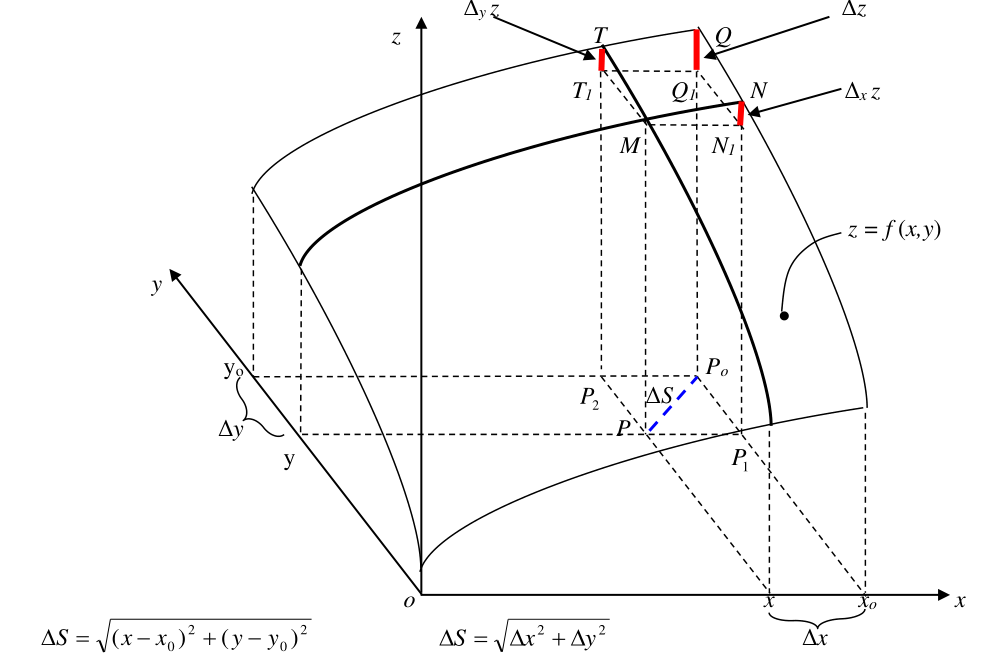
\includegraphics[width=\linewidth]{imagenes/incrementos_de_funcion.png}
	\caption{Imagen sacada de \parencite{am2monllor}. Incrementos de una función}
	\label{fig:inc_funcion}
\end{figure}

Si analizamos la curva \textbf{MN}, que es la intersección de la superficie $ z = f(x,y) $ y el plano $ y = cte $, vemos que si nos movemos sobre ella, $ z $ varía solo en función de $ x $.

Si nos movemos en el eje $ x $ una distancía $ \Delta x $, la variación de $ z $ es lo que se conoce como:

\textbf{Incremento Parcial de $ z $ repecto de $ x $} (es el segmento $\overline{NN_{1}}$ de la figura \ref{fig:inc_funcion})

\centerline{$\boxed{\Delta_{x}z = f(x+\Delta x, y) - f(x,y)}$}

\vspace{0.5cm}
Si en cambio, consideramos a $ x = cte $ y nos vamos moviendo sobre el eje $ y $, la variación de $ z $ es:

\textbf{Incremento Parcial de $ z $ respecto de $ y $} (es el segmento $ \overline{TT_{1}} $ de la figura \ref{fig:inc_funcion})

\centerline{$ \boxed{\Delta_{y}z = f(x, y + \Delta y) - f(x,y)} $}

\vspace{0.5cm}
Si incrementamos simultáneamente a $ x $ en $ \Delta x $, y a $ y $ en $ \Delta y $, obtenemos el:

\textbf{Incremento Total de la función} (segmento $ \overline{QQ_{1}} $ de la figura \ref{fig:inc_funcion}

\section{Límites}
Dada una función $ z = f(x,y) $, se define el límite de esta función cuando $ P(x,y) $ tiende a $ P_{0}(x_{0},y_{0}) $ de la siguiente manera:

"\textit{El límite de $ f(x,y) $ es igual a $ L $ si, para cualquier número $ \varepsilon > 0 $ existe un número $ \delta > 0 $ tal que, si la distancia del punto $ P(x,y) $ a $ P_{0}(x_{0},y_{0}) $ es menor a $ \delta $ entonces, la distancia entre $ f(x,y) $ y $ L $ es menor a $ \varepsilon $, con $ P(x,y) \neq P_{0}(x_{0},y_{0}) $}"
\[
	\lim_{(x,y) \to (x_{0},y_{0})}{f(x,y)} = L \iff \forall \varepsilon > 0 : \exists \delta > 0 \mid 0 < \lVert(x,y) - (x_{0},y_{0})\rVert < \delta \implies \left|f(x,y) - L\right| < \varepsilon
\]

Esta definición implica que por mas pequeño que sea $ \varepsilon{} $ siempre existe una bola reducida $ B_{0}(P_{0},\delta) $ dentro de la cual están los puntos $ P(x,y) $. Se considera una bola reducida porque no nos interesa qué pasa en el punto $ P_{0} $ donde la función puede no estar definida.

Recordemos que cuando estudiabamos límites en análisis I, las trayectorias posibles para acercarse al límite eran dos (por izquierda, y por derecha) y bastaba con probar que los límites de esas dos trayectorias eran iguales para demostrar la existencia del límite en ese punto.

El problema es que ahora, como tenemos dos variables, las trayectorias que existen para acercarse a un mismo punto son infinitas y es imposible calcular el límite de todas las trayectorias para ver si son el mismo.

Una forma de demostrar la existencia de un límite de dos variables es calcularlo aplicando la definición, pero esto se puede volver muy complicado.

Lo que sí podemos hacer se algo parecido a lo que veníamos haciendo para límites de una sola variable, y si llegamos a una indeterminación vemos cómo nos las arreglamos.

\underline{Ejemplo 1}:
\[
	\lim_{(x,y) \to (3,1)}{\left(xy - y^{2}\right)}
\]
En este caso podemos directamente reemplazar $ (x,y) $ por $ (3,1) $ y el resultado es $ L = 2 $. Esto quiere decir que por cualquier camino que nos aproximemos al punto $ P_{0}(3,1) $ los valores de la función van a tender a 2.

En este caso, como no hay problema con ningúna de las variables, decimos que la función tiene Límite Doble y es $ L = 2 $.

\underline{Ejemplo 2}:
\[
\lim_{(x,y) \to (0,0)}{\frac{\sin^{} 3xy}{x}}
\]
En este caso, si evaluamos la función en el $ (0,0) $ tenemos una indeterminación, pero la podemos salvar:
\[
\lim_{(x,y) \to (0,0)}{\frac{\sin^{} 3xy}{x}} = \lim_{(x,y) \to (0,0)}{\frac{3y\sin^{}3xy}{3xy}} = \left(\lim_{(x,y) \to (0,0)}{3y}\right)\times\left(\lim_{(x,y) \to (0,0)}{\frac{\sin^{}3xy}{3xy}}\right) = 0\times1 = 0
\]
Vemos entonces que la función tiene Límite Doble $ L = 0 $.

\underline{Ejemplo 3}:
\[
\lim_{(x,y) \to (0,0)}{\frac{3x^{2}+y}{x^{2}-y}}
\]
En este caso llegamos a una indeterminación si evaluamos la función en el $ (0,0) $ pero no hay forma de salvarla. La forma de saber si existe el límite en estos casos es calcularlo con la definición o fijarnos si aproximandonos por todas las infinitas direcciones obtenemos el mismo resultado. Y no queremos hacer ninguna de las dos cosas.

Entonces, no podemos (o es muy dificil) confirmar la existencia del límite, pero sí puede ser mas sencillo afirmar cuando \textbf{no} existe el mismo, ya que si los límites calculados por dos trayectorias son diferentes, el límite no existe.

Vamos a ver dos formas de hacer esto: usando \textbf{Límites Iterados}, y \textbf{Límites Radiales}.

\subsection{Límites Iterados}
Podemos calcular los límites de una función por trayectorias particulares, denominadas \textbf{Trayectorias Escalonadas}, constituidas por rectas paralelas a los ejes cartesianos y que consiste en llegar al punto $ P_{0} $ partiendo de $ P $ y pasando por $ P_{1} $, y luego hacer lo mismo pero pasando por $ P_{2} $ para comparar los resultados.

\begin{figure}[H]
  \centering
  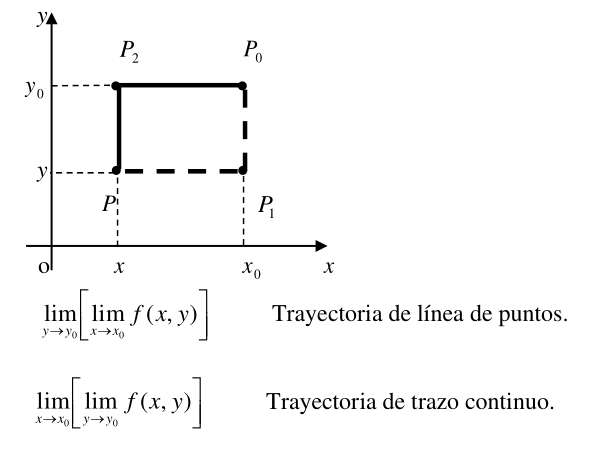
\includegraphics[width=0.5\linewidth]{imagenes/limites_iterados.png}
  \caption{Imagen sacada de \parencite{am2monllor}. Cálculo de límites iterados.}
  \label{fig:limites_iterados}
\end{figure}

\underline{Ejemplo 4}:
Dada $ z = \frac{2x^{2} + y^{3}}{3x^{2} - y^{3}} $, calcular los Límites Iterados en el punto $ P_{0}(0,0) $:
\begin{align*}
	\lim_{y \to 0}{\left[\lim_{x \to 0}{\frac{2x^{2} + y^{3}}{3x^{2} - y^{3}}}\right]} &= -1\\
	\lim_{x \to 0}{\left[\lim_{y \to 0}{\frac{2x^{2} + y^{3}}{3x^{2} - y^{3}}}\right]} &= \frac{2}{3}
\end{align*}

Los Límites iterados son distintos, por lo tanto la función no tiene límite en $ P_{0}(0,0) $.

\fbox{\parbox{0.9\linewidth}{
\textbf{IMPORTANTE}:

Que los límites iterados sean iguales no garantiza que la función tenga límite. Hay que recordar que para que exista el límite en un punto, las infinitas trayectorias a ese punto deben tener el mismo límite, y cuando calculamos los límites iterados solo estamos calculando dos trayectorias. Podría ser que haya una trayectoria con un límite distinto.
}}

\subsection{Límites Radiales}
Consiste entomar el límite siguiendo las trayectorias del haz de rectas que pasan por el punto $ P_{0}(x_{0}, y_{0}) $:

\begin{figure}[H]
  \centering
  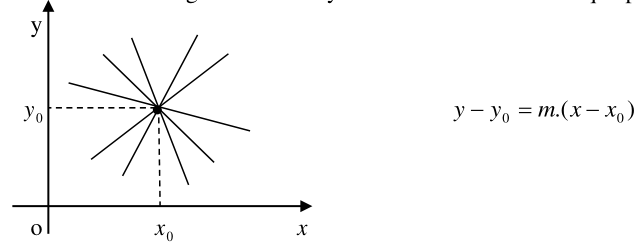
\includegraphics[width=0.5\linewidth]{imagenes/limites_radiales.png}
  \caption{Imagen tomada de \parencite{am2monllor}. Límites radiales}
  \label{fig:limites_radiales}
\end{figure}

Con este método, si $ L $ queda en función de $ m $ significa que tendrá un límite distinto para cada trayectoria, osea que no existe el límite en ese punto.

\underline{Ejemplo 5}:
Dada $ z = \frac{2xy}{3x^{2} - y^{2}} $, calcular el límite de $ z $ en el punto $ P_{0}(0,0) $.
\[
\lim_{(x,y) \to (0,0)}{\frac{2xy}{3x^{2} - y^{2}}}
\]
Como $ P_{0}(0,0) $, sabemos que $ \begin{cases}
  x_{0} = 0 \\
  y_{0} = 0
\end{cases} $, entonces la trayectoria es $ y - 0 = m(x-0) $ que es lo mismo que $ y = mx $.

Ahora como podemos reemplazar $ y $ en función de $ x $, podemos escribir la función y el límite en función de $ x $:
\[
\lim_{x \to 0}{\frac{2x.mx}{3x^{2} - (mx)^{2}}}
\]
Y podemos resolver el límite:
\[
\lim_{x \to 0}{\frac{2x.mx}{3x^{2} - (mx)^{2}}} = \lim_{x \to 0}{\frac{x^{2}2m}{x^{2}(3- (mx)^{2})}} = \frac{2m}{3-m^{2}}
\]

El resultado del límite nos quedó en función de $ m $, así que podemos afirmar que no existe el límite para esa función en el punto $ P_{0}(0,0) $.

Veamos un ejemplo mas:

\underline{Ejemplo 6}:
Dada $ z = \frac{2x^{2}y}{x^{4}+3y^{2}} $, calcular el límite de la función en el punto $ P_{0}(0,0) $

Busquemos primero los límites susecivos:
\begin{align*}
	\lim_{y \to 0}{\left[\lim_{x \to 0}{\frac{2x^{2}y}{x^{4}+3y^{2}}}\right]} &= 0 \\
	\lim_{y \to 0}{\left[\lim_{x \to 0}{\frac{2x^{2}y}{x^{4}+3y^{2}}}\right]} &= 0
\end{align*}

Los límites son iguales, pero habíamos dicho que solo con esta iformación no podíamos afirmar si existe o no el límite.

Calculemos ahora los límites radiales:
 
$
\displaystyle \lim_{(x,y) \to (0,0)}{\frac{2x^{2}y}{x^{4}+3y^{2}}}
\qquad
\begin{cases}
  x_{0} = 0 \\
  y_{0} = 0
\end{cases}
$ la trayectoria es $ y = mx $
\[
\lim_{x \to 0}{\frac{2x^{2}mx}{x^{4}+3(mx)^{2}}} = \lim_{x \to 0}{\frac{2mx}{x^{2}+3m^{2}}} = 0
\]

Obtuvimos el mismo valor de límite a lo largo de cualquier trayectoria paralela a los ejes coordenados (límites iterados) y de cualquier recta que pase por el origen. \textbf{Pero esto NO demuestra que el límite de la función sea 0}, porque hay infinitas trayectorias que hay que analizar y no las analizamos todas. Por ejemplo, analicemos la trayectoria de la parábola $ y = x^{2} $, y veamos si el límite nos sigue dando 0.
\[
	\lim_{(x,y) \to (0,0)}{\frac{2x^{2}y}{x^{4}+3y^{2}}} =\lim_{(x,y) \to (0,0)}{\frac{2x^{2}x^{2}}{x^{4}+3(x^{2})^{2}}} = \lim_{(x,y) \to (0,0)}{\frac{2x^{4}}{x^{4}+3x^{4}}} = \frac{1}{2}
\]

Obtuvimos un valor distinto de límite, por lo tanto el límite para esta función cuando $ P $ tiende a $ (0,0) $ NO EXISTE.

\textbf{Estos métodos no sirven para demostrar si existe el límite, solo nos sirven para demostrar cuándo la funcion NO lo tiene.}

\section{Continuidad}
Es lo mismo que siempre. Sea la función $ z = f(x,y) $ y $ P_{0}(x_{0}, y_{0}) $, $ z $ es continua en $ P_{0} $ si:
\[
\lim_{(x,y) \to (x_{0},y_{0})}{f(x,y)} = f(x_{0},y_{0})
\]

Para que se cumpla esto se tiene que cumplir tres condiciones básicas:
\begin{enumerate}[1.]
  \item Que el límite exista para $ P(x,y) \to P_{0}(x_{0},y_{0}) $

  \item Que la función esté definida en $ P_{0}(x_{0},y_{0}) $

  \item Que el límite de la función es igual al valor de la función en $ P_{0}(x_{0},y_{0}) $
\end{enumerate}

Si la igualdad no se cumple en $ P_{0} $ quiere decir que este es un \textbf{punto de discontinuidad}.

Si no existe el límite en ese punto, la discontinuidad es \textbf{esencial}.

Si existe el límite, pero la función no es continua, la discontinuidad es \textbf{evitable}. Lo que se hace es redefinir la función para que sea continua.

\section{Derivadas Parciales}
Sea la función $ z = f(x,y) $, de dos variables independientes, y consideremos que se mantiene a $ y $ constante, haciendo variar solamente a $ x $, encontes la función planteada se comporta como una función \textbf{derivada parcial de la función con respecto a "$ x $"}, que se expresa así:
\[
\pdv[]{f(x,y)}{x} = \lim_{\Delta x \to 0}{\frac{\Delta_{x}f(x,y)}{\Delta x}} = \lim_{\Delta x \to 0}{\frac{f(x + \Delta x,y) - f(x,y)}{\Delta x}}
\]

Otras formas de escribir la derviada parcial son las siguientes:
\[
\pdv[]{f(x,y)}{x} = \pdv[]{z}{x} = \pdv[]{f}{x} = z_{x}^\prime = f_{x} = \dots
\]

De igual manera, podemos mantener constante a $ x $ y derivar a la función para obtener la \textbf{derivada parcial respecto de "$ y $"}
\[
\pdv[]{f(x,y)}{y} = \lim_{\Delta y \to 0}{\frac{\Delta_{y}f(x,y)}{\Delta y}} = \lim_{\Delta y \to 0}{\frac{f(x,y + \Delta y) - f(x,y)}{\Delta y}}
\]

La forma de calcular estas derivadas es la misma que usabamos cuando teníamos una sola variable, solo que ahora hay que tener en cuenta que si estamos haciendo la derivada parcial respecto de $ x $, la variable $ y $ es una constante y la tenemos que tratar como tal.

\underline{Ejemplos}:
\begin{enumerate}[1.]
  \item Las derivadas parciales de la funcion $ z = y^{3}\cos^{}x $ son: 
	$
	\begin{cases}
	  \pdv[]{z}{x} = -y^{3}\sin^{}x \\
	  \pdv[]{z}{y} = 3y^{2}\cos^{}x
	\end{cases}
	$

  \item Calcular las derivadas parciales de la función $ z = 3x^{2}y - y^{2} $ en el punto $ P(1,2) $:
\begin{align*}
	\pdv[]{f(x,y)}{x} & = 6xy & \pdv[]{f(1,2)}{x} & = 12 \\ 
	\pdv[]{f(x,y)}{y} & = 3x^{2} - 2y & \pdv[]{f(1,2)}{y} & = -1 
\end{align*}
	  
\end{enumerate}


\subsection{Interpretación geométrica de las derivadas parciales}
Consideremos a la función $ z = 4 - x^{2} - 2y^{2} $ y busquemos sus derivadas parciales en los puntos $ P_{0}(1,1) $.

Tenemos que:
\begin{align*}
	\pdv[]{f(x,y)}{x} &= -2x &= \pdv[]{f(x,y)}{y} &= -4y\\
	\pdv[]{f(1,1)}{x} &= -2 &= \pdv[]{f(1,1)}{y} &= -4
\end{align*}

Si miramos la figura \ref{fig:derivada_parcial_x}, podemos que ver cuando hacemos la derivada parcial respecto de x, nos estamos moviendo en el plano $ y = 1 $, y la derivada parcial es la pendiente de la recta tangente a la curva generada por la función $ z $ en la intersección con ese plano $ y = 1 $.

\begin{figure}[H]
  \centering
  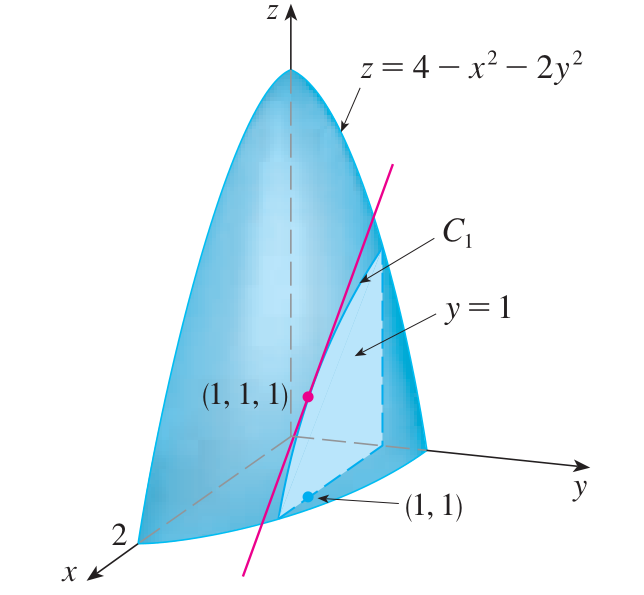
\includegraphics[width=0.3\linewidth]{imagenes/interp_geom_derivada_paracial_x.png}
  \caption{Imagen sacada de \parencite{stewart2}. Derivada parcial respecto de $ x $.}
  \label{fig:derivada_parcial_x}
\end{figure}

Lo mismo podemos observar cuando analizamos la figura \ref{fig:derivada_parcial_y}. En este caso, el plano sobre el que nos movemos es $ x = 1 $, y la derivada parcial es la pendiente de la recta tangente a la curva generada por la intersección de la función $ z $ con él.

\begin{figure}[H]
  \centering
  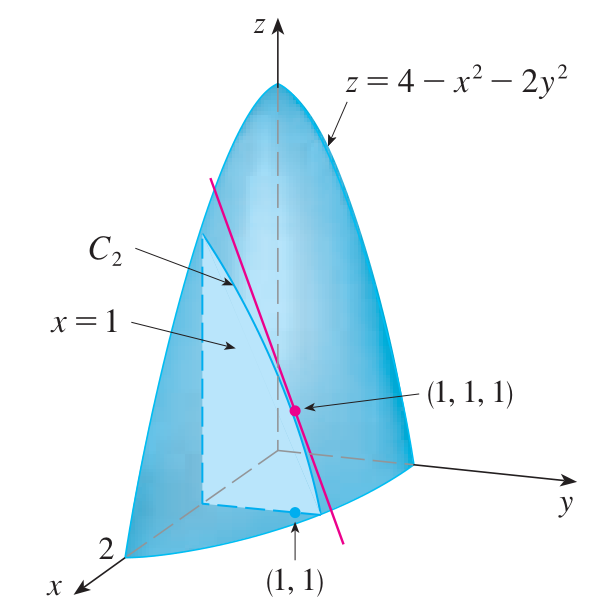
\includegraphics[width=0.3\linewidth]{imagenes/interp_geom_derivada_paracial_y.png}
  \caption{Imagen sacada de \parencite{stewart2}. Derivada parcial respecto de $ y $.}
  \label{fig:derivada_parcial_y}
\end{figure}

\subsection*{Derivavilidad de una función}
Una función de varias variables independientes es derivable en un punto si es continua en ese punto.

\subsection{Derivadas parciales sucesivas}
Igual que con las derivadas normales, una derivada parcial la podemos derivar cuantas veces queramos obteniendo derivadas parciales segundas, terceras, etc., con respecto a cada una de las variables consideradas.

Así para una función de dos variables independientes sus derivadas parciales son:
\begin{align*}
	z &= f(x,y) & z &= x^{4}\sin^{}5y\\
	\pdv[]{z}{x} &= f_{x}^{\prime}(x,y) & \pdv[]{z}{x} &= 4x^{3}\sin^{}5y\\
	\pdv[]{z}{y} &= f_{y}^{\prime}(x,y) & \pdv[]{z}{y} &= 5x^{4}\cos^{}5y
\end{align*}

Estas pueden ser derivadas nuevamente obteniendo las derivadas parciales de segundo orden:
\begin{align*}
	\pdv[2]{z}{x} &= f_{xx}^{\prime\prime}(x,y) & \pdv[2]{z}{x} &= 12x^{2}\sin^{}5y\\
	\pdv[2]{z}{y}{x} &= f_{xy}^{\prime\prime}(x,y) & \pdv[2]{z}{y}{x} &= 20x^{3}\cos^{}5y\\
	\pdv[2]{z}{x}{y} &= f_{yx}^{\prime\prime}(x,y) & \pdv[2]{z}{x}{y} &= 20x^{3}\cos^{}5y\\
	\pdv[2]{z}{y} &= f_{yy}^{\prime\prime}(x,y) & \pdv[2]{z}{y} &= -25x^{4}\sin^{}5y
\end{align*}

Y así siempre que existan las derivadas correspondientes, se pueden seguir derivando de forma sucesivas.

Estas derivadas parciales sucesivas vemos que no son todas distintas entre sí. Hay un teorema que dice que: "\textit{Si las derivadas sucesivas a calcular son continuas, el orden de derivación no altera la derivada, siempre que la cantidad de veces que se derive respceto a cada variable sea la misma}."

Es decir, que si derivamos primero respecto a $ x $ y luego respecto a $ y $, o primero respecto a $ y $ y luego respecto a $ x $, SIEMPRE QUE TODAS LAS DERIVADAS QUE CALCULAMOS SEAN CONTINUAS vamos a llegar al mismo resultado.

Esto se puede demostrar con el teorema de Schwartz, pero no lo vemos en clase.

\subsection{Diferencial}
Para explicar qué es el diferencial vamos a volver a trabajar con funciones de $ \mathbb{R}^{}\to\mathbb{R}^{} $ y después vamos a aplicar los conocimientos en las funciones de $ \mathbb{R}^{n}\to\mathbb{R}^{m} $.

La notación diferencial en realidad la venimos viendo hace un montón pero nunca supimos de dónde venía ni qué significaba. La veíamos por ejemplo cuando estudiabamos derivadas, que podiamos expresarla como $ \dv[]{y}{x} $ donde $ y = f(x) $. También la veíamos en las integrales de la forma $ \int_{}^{} f(x) \,dx $. Esto lo tomabamos como que solo era una notación, pero en realidad no, $ dx $ y $ dy $ son dos variables que tienen la propiedad de que cuando su razón existe, esta es igual a la derivada.

\fbox{\parbox{0.9\linewidth}{
\textbf{Definición de diferenciales}

Sea $ y = f(x) $ una función derivable. La \underline{diferencial $ dx $} es una variable independiente. La \underline{diferencial $ dy $} es
\[
dy = f^{\prime}(x)dx
\]
}}\vspace{0.2cm}

Como $ dx $ es una variable independiente puede tomar cualquier valor, pero el valor de $ dy $ va a depender tanto del valor que tome la variable $ dx $ como del de la variable $ x $.

\subsubsection{Interpretación geométrica del diferencial}
En la siguiente figura podemos ver gráficamente a qué llamamos $ dx $ y $ dy $.

\begin{figure}[H]
  \centering
  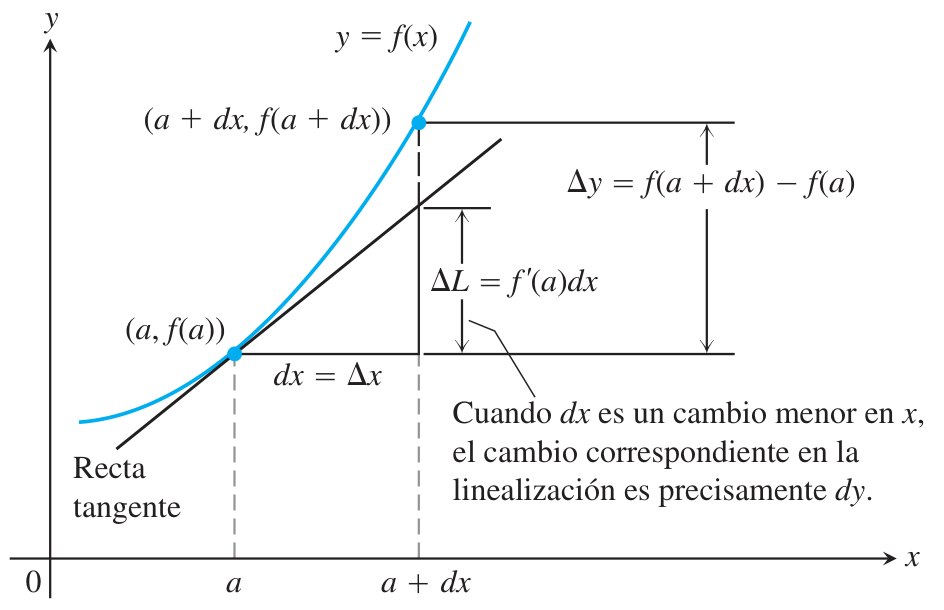
\includegraphics[width=0.5\linewidth]{imagenes/interp_geom_diferencial.png}
  \caption{Imagen sacada de \parencite{thomas_calc_uv}. Interpretación geométrica del diferencial.}
  \label{fig:interp_geom_diferencial}
\end{figure}

Vemos en la figura \ref{fig:interp_geom_diferencial} que la diferencial $ dy $ es el cambio $ \Delta L $ cuando $ x = a $ cambia en una cantidad $ dx = \Delta x $. Y lo podemos comprobar de la siguiente forma:
\begin{align*}
  \Delta L &= L(a + dx) - L(a)\\
  \Delta L &= \underbrace{f(a) + f^{\prime}(a)\left[(a + dx) - a\right]}_{L(a + dx)} - \underbrace{f(a)}_{L(a)}\\
  \Delta L &= f^{\prime}(a)dx
\end{align*}

Entonces, $ \Delta L = dy $ y representa la magnitud que se eleva o baja la recta tangente cuando $ x $ cambia en una cantidad $ dx = \Delta x $.

Si $ dx \neq 0 $, entonces el cociente de la diferencial $ dy $ entre la diferencial $ dx $ es igual a la derivada $ f^{\prime} (x,y) $.

Si tenemos la ecuación $ f(x) = 3x^{2} - 6 $, entonces $ dy = f^{\prime}(x)dx = 6xdx $.

Toda fórmula de derivación como 
\begin{align*}
	\dv[]{(u + v)}{x} &= \dv[]{u}{x} + \dv[]{v}{x} && \text{o} & \dv[]{(\sin^{}u)}{x} &= \cos^{}u\dv[]{u}{x}
\end{align*}

Tiene una forma diferencial correspondiente como 
\begin{align*}
	d(u+v) &= du+dv && \text{o} & d(\sin^{}u) &= \cos^{}udu
\end{align*}

\subsubsection{Estimación con diferenciales}
\fbox{\parbox{0.9\linewidth}{
\textbf{Aclaraciones}


Acá me mezclo un poco así que vamos a hacer un par de aclaraciones.
\begin{itemize}
  \item $ \Delta y $ es lo que varía la función $ f(x) $ si nos movemos una distancia $ \Delta x = dx $ sobre el eje $ x $. La variación de la función se calcula como cualquier variación, punto final menos inicial:
\[
\Delta y = f(a + dx) - f(a)
\]

  \item $ dx = \Delta x $ y es la distancia que nos movemos en el eje $ x $.

  \item Cuando $ \Delta x $ es pequeña, podemos decir (y se vé en la gráfica de la figua \ref{fig:interp_geom_diferencial}) que $ dy $ es aproximadamente igual a $ \Delta y $. Osea,
\[
	\Delta y \approx dy
\]

  \item $ dy $ \textbf{no es} $ \Delta y $, solo es aproximadamente igual cuando $ dx $ es muy pequeño.
La fórmula de $ dy $ es:
\[
dy = f^{\prime}(x)dx
\]
\end{itemize}
}}\vspace{0.2cm}

Ahora sí, supongamos que conocemos el valor de una función derivable $ f(x) $ en un punto $ a $ y necesitamos estimar cuánto cambiará este valor en $ f(a + dx) $. Si $ dx = \Delta x $ es pequeña, mirando la figura \ref{fig:interp_geom_diferencial}, podemos ver que $ \Delta y $ es aproximadamente igual a $ dx $.

Sabemos que $ \Delta y = f(a + dx) - f(a) $, entonces $ f(a + dx) = f(a) - \Delta y $. Y recién dijimos que para valores muy chicos de $ dx $, $ \Delta y $ era aproximadamente igual a $ dy $ así que podemos decir que
\[
	f(a + dx) \approx f(a) + dy
\]
que es lo mismo que decir 
\[
dy \approx f(a + dx) - f(a)
\]
Entonces podemos usar $ dy $ para estimar $ f(a + dx) $ cuando conocemos $ f(a) $ y los valores de $ dx $ son pequeños.

\subsubsection{Error en la aproximación diferencial}
Sea $ f(x) $ derivable en $ x = a $ y supongamos que $ dx = \Delta x $ es un incremento de $ x $. Tenemos dos formas de describir el cambio en $ f $ cuando $ x $ cambia de $ a $ a $ a + \Delta x $:

El cambio real: $ \Delta f = f(a + \Delta x) - f(a) $

La estimación diferencial: $ df = f^{\prime}(a)\Delta x $

¿Qué tan bien aproxima $ df $ a $ \Delta f $?

Podemos medir el error de la aproximación si restamos $ df $ de $ \Delta f $:

\begin{align*}
  \text{Error de aproximacion} &= \Delta f - df \\
   &= \Delta f - f^{\prime}(a)\Delta x\\
    &= \underbrace{f(a + \Delta x) - f(a)}_{\Delta f} - f^{\prime}(a)\Delta x\\
    &= \underbrace{\left(\frac{f(a + \Delta x) - f(a)}{\Delta x} - f^{\prime}(a)\right)}_{\text{A esta parte la llamamos }\varepsilon}\Delta x\\
     &= \varepsilon \Delta x
\end{align*}

Cuando $ \Delta x \to 0 $, el cociente de diferencias 
\[
\frac{f(a + \Delta x) - f(a)}{\Delta x}
\]
se aproxima a la derivada $ f^{\prime}(a) $ así que la cantidad entre paréntesis se vuelve un número muy pequeño. Es decir, cuando $ \Delta x \to 0 $, $ \varepsilon \to 0 $.

Ahora podemos afirmar lo siguiente:
\[
\underbrace{\Delta f}_{\text{cambio real}} = \underbrace{f^{\prime}(a)\Delta x}_{cambio estimado} + \underbrace{\varepsilon \Delta x}_{error}
\]


\subsection{Diferencial en funciones de varias variables}
\subsubsection{Repaso}
Recordemos el teorema del valor medio, que dice que:

\fbox{\parbox{0.9\linewidth}{
\textbf{Teroema del Valor Medio} \\
Si $ f $ es una función que satisface las siguientes hipótesis
\begin{enumerate}[1.]
	\item $ f $ es continua sobre el intervalo cerrado $ [a,b] $

	\item $ f $ es derivable sobre el intervalo abierto $ (a,b) $
\end{enumerate}
entonces existe un número $ x = c $ en $ (a,b) $ tal que:
\[
	f^{\prime}(c) = \frac{f(b) - f(a)}{b - a}
\]
o, equivalentemente
\[
	f(b) - f(a) = f^{\prime}(c)(b - a)
\]
}}
\vspace{0.2cm}

Basicamente, lo que dice es que si $ f $ es continua y derivable dentro de un intervalo, entonces hay al menos un punto dentro de ese intervalo en el que la derivada de la función es igual a la pendiente de la recta secante que va de $ f(a) $ a $ f(b) $.

\begin{figure}[H]
  \centering
  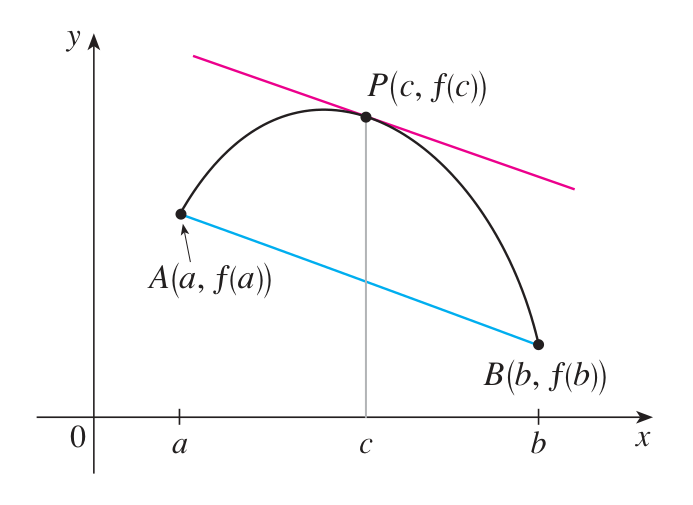
\includegraphics[width=0.5\linewidth]{imagenes/valor_medio.png}
  \caption{Imagen sacada de \parencite{stewart2}. Teorema del Valor Medio}
  \label{fig:valor_medio}
\end{figure}



\subsection{Diferencial total}
Dada una función $ z = f(x,y) $, vimos en la sección \ref{sec:incrementos_func} que su incremento total es:
\[
\Delta z = f(x + \Delta x, y + \Delta y) - f(x,y)
\]

Supongamos que la función es continua y tiene derivadas parciales también continuas en el punto considerado.

A la expresion del incremento total le sumamos y restamos $ f(x + \Delta x,y) $ y la reordenamos un poquito:
\[
\Delta z = \underbrace{f(x + \Delta x, y) - f(x,y)}_{\Delta z_{1}} + \underbrace{f(x + \Delta x, y + \Delta y) - f(x + \Delta x, y)}_{\Delta z_{2}}
\]

A los primeros dos términos de la ecuación los podemos considerar como un $ \Delta z_{1} $, que simboliza el incremento de $ z $ al movernos desde el punto $ f(x,y) $ hasta el punto $ f(x + \Delta x, y) $. Osea, que nos movimos en un plano paralelo al eje $ x $ con $ y = cte $.

A los últimos dos términos los podemos considerar como un $ \Delta z_{2} $, que es ahora el incremento de $ z $ al movernos desde el punto final anterior $ f(x + \Delta x, y) $ hasta el punto $ f(x + \Delta x, y + \Delta y) $. En este caso nos movemos sobre un eje paralelo al eje $ y $, manteniendo $ x = cte $.

Lo que estamos haciendo es calcular el incremento real de $ z $ pero en dos partes. Primero nos movemos una distancia $ \Delta x $ con $ y = cte $, y luego desde ese punto en el que quedamos nos movemos una distancia $ \Delta y $ con $ x = cte $.

Ahora, en $ z_{1} $, como estamos considerando que $ y=cte $ podemos aplicar el Teorema del Valor Medio sobre ese plano. Este teorema nos dice que existe un valor $ c $ entre $ x $ y $ x + \Delta x $ donde
\[
	f(x + \Delta x, y) - f(x,y) = f_{x}(c,y)\Delta x
\]


Y podemos hacer lo mismo en $ z_{2} $ ya que $ x = cte $. En este caso el Teorema del Valor medio nos dice que existe un número $ d $ entre $ y $ y $ y + \Delta y $ donde
\[
	f(x + \Delta x, y + \Delta y) - f(x + \Delta x, y) = f_{y}(x,d)\Delta y
\]

Entonces la ecuación del incremento de $ z $ queda así: 

\[
	\Delta z = f_{x}(c, y)\Delta x + f_{y}(x + \Delta x, d)\Delta y
\]

\begin{figure}[H]
  \centering
  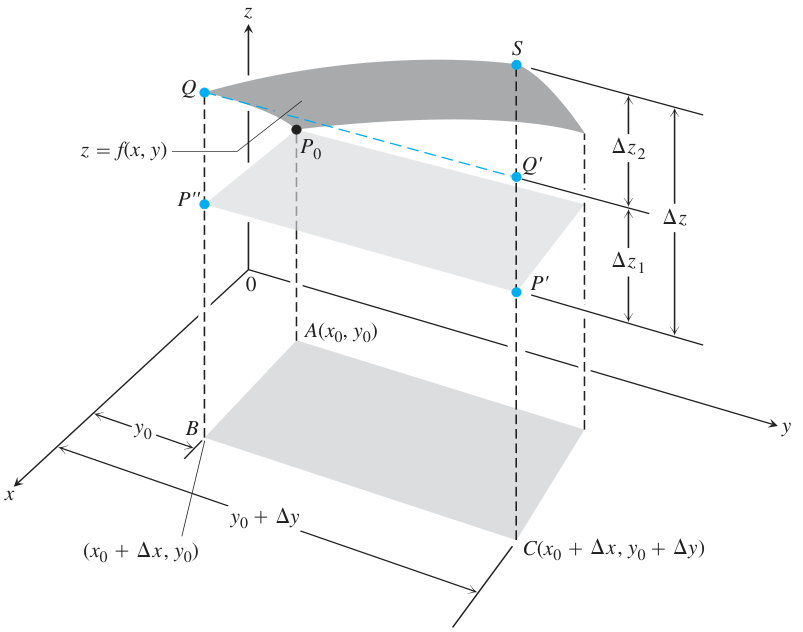
\includegraphics[width=0.7\linewidth]{imagenes/incremento_total.png}
  \caption{Imagen sacada de \parencite{thomas_calc_vv}}
  \label{fig:incremento_total}
\end{figure}

Miremos la figura \ref{fig:incremento_total}. Lo que acabamos de hacer en cuentas lo podemos explicar graficamente de la siguiente forma. 

Partimos del punto $ P_{0} $ que sería nuestro $ f(x,y) $. De ahí, lo que habíamos hecho era movernos sobre el eje $ x $ una distancia $ \Delta x $ manteniendo un $ y = cte $, que sería lo mismo que movernos desde $ P_{0} $ hacia $ P^{\prime\prime} $. Esto representaría el incremento del $ z_{1} $ que habíamos identificado antes. Ese incremento sería el módulo del segmento $ \overline{P^{\prime\prime}Q} $.

Después lo que habíamos hecho fue movernos desde ese último punto en el que habíamos quedado, pero ahora nos movíamos sobre el eje $ y $ mientras manteníamos un $ x = cte $. En el gráfico sería el equivalente a partir del punto $ P^{\prime\prime} $ e ir hacía el punto $ P^{\prime} $. Esto sería el incremento $ z_{2} $, que en el gráfico es el módulo del segmento $ \overline{Q^{\prime}S} $.

Entonces ahora es mas facil ver que cuando sumamos esos dos incrementos, estamos obteniendo el valor real del incremento total de $ z $.

Esto es buenísimo, pero en realidad nosotros queríamos calcular el diferencial total, no el incremento total. Y acá pasa lo mismo que pasa cuano teníamos una sola variable, solo que ahora tenemos dos. Entonces ahora, $ dx $ y $ dy $ son las variables independientes, y $ dz $ es la variable dependiente.

Para una variable habíamos dicho que cuando $ dx $ era muy chico, se cumplía que $ dy \approx \Delta y $ y ahora pasa lo mismo. Podemos decir que $ dz \approx \Delta z $ cuando $ dx \to 0 $ y $ dy \to 0 $.

Analicemos entonces la función que obtubimos del incremento total cuando $ \Delta x \to 0 \land \Delta y \to 0 $.
Como $ c $ es un valor que está entre $ (x, x + \Delta x) $ y $ d $ es un valor entre $ (y, y + \Delta y) $, sabemos que cuando $ \Delta x \to 0 $ y $ \Delta y \to 0 $, $ c \to x $ y $ d \to y $. Pero estos valores no son exactamente $ x $ e $ y $. Son una aproximación, pero con esa aproximación viene un error. 
\begin{align*}
  \varepsilon_{1} &= f_{x}(x,y) - f_{x}(x,y)\\
  \varepsilon_{2} &= f_{y}(x + \Delta x, d) - f_{y}(x,y)
\end{align*}

Entonces ahora podemos decir lo siguiente:
\begin{align*}
  \Delta z &= \Delta z_{1} + \Delta z_{2} \\
   &= f_{x}(c,y)\Delta x - f_{y}(x + \Delta x, d)\Delta y \\
    &= \left[f_{x}(x,y) + \varepsilon_{1}\right]\Delta x + \left[f_{y}(x,y) + \varepsilon_{2}\right]\Delta y \\
    \Delta z &= f_{x}(x,y)\Delta x + f_{y}(x,y)\Delta y + \varepsilon_{1}\Delta x + \varepsilon_{2}\Delta y
\end{align*}

La suma de los dos primeros términos recibe el nombre de parte principal del incremento y es el \textbf{Diferencial Total} de la función:
\[
\boxed{dz = f_{x}(x,y)\Delta x + f_{y}(x,y)\Delta y}
\]
También se puede expresar:
\[
\boxed{dz = \pdv[]{z}{x}dx + \pdv[]{z}{y}dy}
\]
Esto que acabamos de demostrar acá sirve para funciones de $ n $ variables:

\underline{Ejemplo:}

Calculemos el diferencial total de la función $ z = 2x^3y^2 $, en el punto $ P(1,2) $, para cuando la variable independiente $ x $ se incrementa en $ dx=0,03 $ y la variable independiente $ y $ se incrementa en $ dy=0,02 $.
\begin{align*}
  df(x,y) &= 6x^2y^2dx+4x^3ydy\\
  df(1,2) &= 6\cdot 1^2\cdot 2^2\cdot 0,03+4\cdot 1^3\cdot 2\cdot 0,02\\
  df(1,2) &= 0,88
\end{align*}

Significa que cuando las variables independientes $ x $ e $ y $ se incrementan en $ dx = 0.02 $ y en $ dy=0.03 $ respectivamente, la función se incrementa aproximadamente en $ dz=0.88 $.


\subsection{Plano tangente y recta normal a una superficie}
% Recordemos que 
%
% Dada la función $ z = f(x,y) $ sabemos que su diferencial es:
% \[
% 	dz = \pdv[]{f(x,y)}{x}dx + \pdv[]{f(x,y)}{y}dy
% \]
%
% Si ahora consideramos que $ \Delta x = x - x_{0} $ y $ \Delta y = y- y_{0} $, entonces $ dz = z - z_{0} $. 
%
% Esto lo podemos reemplazar en la ecuación del diferencial para obtener: 
% \[
% z - z_{0} = \pdv[]{f(x_{0}, y_{0})}{x} \left(x-x_{0}\right) + \pdv[]{f(x_{0}, y_{0})}{y}\left(y - y_{0}\right)
% \]
%
% que es la ecuación de un plano que pasa por el punto $ M(x_{0},y_{0},z_{0}) $.
%
% Para verlo mejor podemos reescribir la ecuación de la siguiente forma:
% \[
% \underbrace{1}_{-C}\left(z-z_{0}\right) = \underbrace{\pdv[]{f(x_{0},y_{0})}{x}}_{A}\left(x-x_{0}\right)+\underbrace{\pdv[]{f(x_{0},y_{0})}{y}}_{B}\left(y-y_{0}\right)
% \]
% \[
% \begin{aligned}
%   \underbrace{\pdv[]{f(x_{0},y_{0})}{x}\left(x-x_{0}\right)}_{A}+\underbrace{\pdv[]{f(x_{0},y_{0})}{y}\left(y-y_{0}\right)}_{B}+\underbrace{\left(-1\right)}_{C}\left(z-z_{0}\right) &= 0\\
%   \left(\pdv[]{f(x_{0},y_{0})}{x},\pdv[]{f(x_{0},y_{0})}{y},-1\right)\cdot \left(x-x_{0},y-y_{0},z-z_{0}\right) &= 0\\
% \end{aligned}
% \]
% \[
%   \vv{n_{\pi}}\cdot \vv{P_{0}P} = 0
% \]
Recordemos algo de teoría primero. Sabemos que la ecuación de un plano está dada por el producto escalar entre un vector normal al plano y un punto cualquiera del mismo.
\[
\pi = \vv{n_{\pi}}\cdot \vv{P_{0}P} = 0
\]

donde $ \vv{n_{\pi}} = \left(A,B,C\right) $ y $ \vv{P_{0}P} = \left(x-x_{0},y-y_{0},z-z_{0}\right) $. Si desarrollamos esta ecuación obtenemos lo siguiente
\[
A\left(x-x_{0}\right) + B\left(y-y_{0}\right) + C\left(z-z_{0}\right) = 0
\]

Al dividir esta ecuación por $ C $, podemos decir que $ a = -A/C $ y que $ b = -B/C $, y de esta manera podemos reescribir la ecuación anterior como sigue

\begin{equation}\label{eq:plano-tg}
z-z_{0} = a\left(x-x_{0}\right) + b\left(y-y_{0}\right)
\end{equation}

Quedemonos con esto en la cabeza porque lo vamos a usar enseguida, pero primero tenemos que llegar hasta ahí. Imaginemos que tenemos una superficie $ S $ dada por la ecuación $ z=f(x,y) $, donde $ f $ tiene primeras derivadas parciales continuas. Habíamos visto mas arriba que cuando calculabamos las derivadas parciales de una función, lo que hacíamos era analizar las curvas dadas por la intersección de dicha función con los planos verticales $ y=y_{0} $ y $ x=x_{0} $, y el resultado era la pendiente de la recta tangente a dicha curva. Vamos a llamar $ T_{1} $ a la recta tangente a la curva dada por la intersección de $ z $ con el plano $ y =y_{0} $, y $ T_{2} $ a la recta tangente a la curva dada por la intersección de $ z $ con el plano $ x=x_{0} $. También vamos a definir al punto $ P(x_{0}, y_{0}, z_{0}) $ como el punto que se encuentra sobre la superficie $ S $; notar que al tener coordenadas $ x_{0} $ y $ y_{0} $ este punto se encuentra en la intersección de las rectas $ T_{1} $ y $ T_{2} $. (Ver Figura \ref{fig:plano-tg})
\begin{figure}[H]
  \centering
  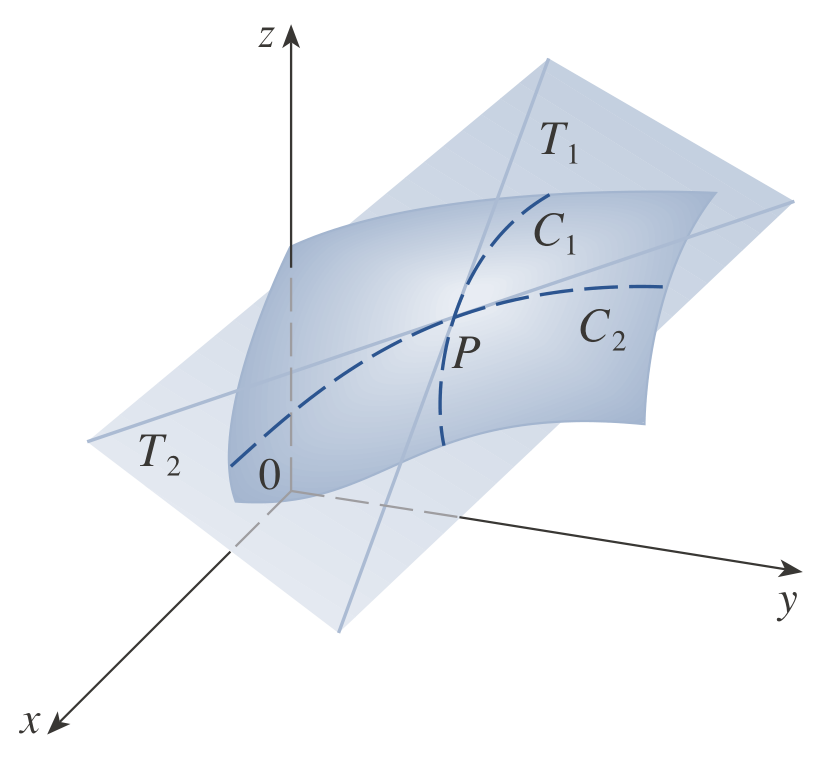
\includegraphics[width=0.5\linewidth]{imagenes/plano-tg.png}
  \caption{Imagen sacada de \parencite{stewart2}. El plano tangente contiene a las rectas $ T_{1} $ y $ T_{2} $.}
  \label{fig:plano-tg}
\end{figure}

En la Figura \ref{fig:plano-tg} podemos ver que el \textbf{plano tangente} a la función $ z=f(x,y) $ en el punto $ P $ es el plano que contiene a las dos rectas tangentes $ T_{1} $ y $ T_{2} $.

Ahora sí, volvamos a la ecuación \ref{eq:plano-tg} y analicémosla. Si dicha ecuación representa el plano tangente en el punto $ P(x_{0},y_{0},z_{0}) $, su intersección con el plano $ y=y_{0} $ tiene que ser la recta tangente $ T_{1} $. Al calcular esta intersección obtenemos
\[
z-z_{0} = a\left(x-x_{0}\right)
\]

Vemos que esta es la ecuación de una recta con pendiente $ a $, pero habíamos dicho recién que la pendiente de esta recta era tangente a la función $ z=f(x_{0},y_{0}) $ por lo que $ a=f_{x}(x_{0},y_{0}) $.

De forma análoga, si hacemos la intersección con el plano $ x=x_{0} $ obtenemos $ z-z_{0}=b\left(y-y_{0}\right) $, que representa a la recta $ T_{2} $, así que $ b=f_{y}(x_{0},y_{0}) $.

Ahora que sabemos todo esto podemos afirmar lo siguiente:

\vspace{0.2cm}
\fbox{\parbox{0.9\linewidth}{
\textbf{Ecuación del plano tangente}

Si una función $ f $ tiene derivadas parciales continuas, una ecuación del plano tangente a la superficie $ z=f(x,y) $ en el punto $ P(x_{0},y_{0},z_{0}) $ es
\[
z-z_{0}=f_{x}(x_{0},y_{0})\left(x-x_{0}\right) + f_{y}(x_{0},y_{0})\left(y-y_{0}\right)
\]
}}\vspace{0.2cm}

\underline{Ejemplo 1:}

Determinar las ecuaciones del Plano Tangente y la Recta Normal a la superficie $ z = 9 - x^2 - y^2 $ en el punto $ M(1,2,4) $.

\begin{align*}
	z - z_{0} = \pdv[]{f(x_{0}, y_{0})}{x} \left(x-x_{0}\right) + \pdv[]{f(x_{0}, y_{0})}{y}\left(y - y_{0}\right) && \text{Ecuación del Plano Tangente}\\[0.2cm]
	z - 4 = \pdv[]{f(1, 2)}{x} \left(x-1\right) + \pdv[]{f(1, 2)}{y}\left(y - 2\right)&&\\[0.2cm]
	\pdv[]{f(x,y)}{x} = -2x \quad \to \quad \pdv[]{f(1,2)}{x}  = -2&&\\[0.2cm]
	\pdv[]{f(x,y)}{y} = -2y \quad \to \quad \pdv[]{f(1,2)}{y}  = -4&&\\[0.2cm]
	z-4 = -2\left(x-1\right) - 4\left(y-2\right)  \to \boxed{2x+4y+z=14} && \text{Plano Tangente}\\[0.2cm]
	\frac{x-1}{2} = \frac{y-2}{4} = \frac{z-4}{1} &&\text{Recta Normal}
\end{align*} 

\underline{Ejemplo 2:}

Determinar el plano tangente al paraboloide elíptico $ z=2x^2 - y^2 $ en el punto $ (1,1,3) $.

Armamos nuesetra función: $ f(x,y)=2x^2+y^2 $

Calculamos sus derivadas paraciales:
\begin{align*}
	f_{x}(x,y) &= 4x && \to & f_{x}(1,1) &= 4\\
	f_{y}(x,y) &= 2y && \to & f_{y}(1,1) &= 2
\end{align*}

Entonces la ecuación del plano tangente es:
\begin{align*}
  z-3 &= 4\left(x-1\right)+2\left(y-1\right)\\
  z &= 4x+2y-3
\end{align*}

\begin{figure}[H]
  \centering
  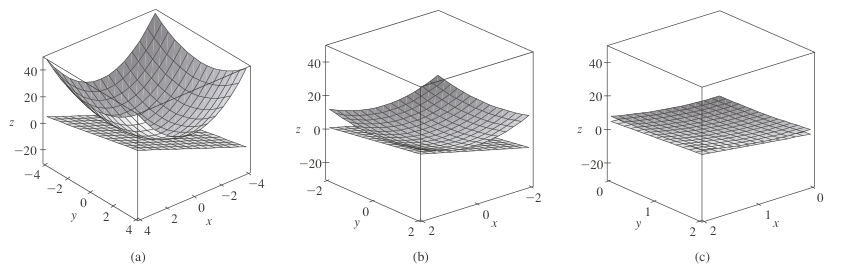
\includegraphics[width=\linewidth]{imagenes/aprox-lineal.png}
  \caption{Imagen sacada de \parencite{stewart2}. Plano tangente a $ z=2x^2+y^2 $}
  \label{fig:aprox-lineal}
\end{figure}

Si prestamos atención a la Figura \ref{fig:aprox-lineal} podemos ver que a medida que nos acercamos al punto $ (1,1,3) $, la función y su plano tangente en dicho punto se asemejan cada vez mas. Podemos decir entonces que la función lineal de dos variables
\[
L(x,y)=4x+2y-3
\]

es una buena aproximación a $ f(x,y)=2x^2+y^2 $ cuando estamos en una bola alrededor del punto $ (1,1,3) $. La función $ L $ se llama \textit{linealización} de $ f $ en $ (1,1) $ y la aproximación 
\[
f(x,y) \approx 4x+2y-3
\]

se llama \textbf{aproximación lineal} del plano tangente de $ f $ en $ (1,1) $.

\subsection{La regla de la cadena}
La regla de la cadena funciona de manera similar a como lo hacía cuando trabajabamos con funciones reales, solo que ahora al tener mas variables se agregan algunas cosas. La regla conviene explicarla en dos casos separados y después presentar el caso general que aplica para cualquier función $ f:\mathbb{R}^{n} \to \mathbb{R}^{m} $.
\subsubsection{Caso 1}
Supongamos que $ z=f(x,y) $ es una función derivable de $ x $ y $ y $, donde $ x=g(t) $ y $ y=h(t) $ son funciones derivables de $ t $. Entonces, $ z $ es una funcion derivable de $ t $ y
\[
\dv[]{z}{t} = \pdv[]{f}{x}\dv[]{x}{t} + \pdv[]{f}{y}\dv[]{y}{t}
\]

\underline{Ejemplo:}

Si $ z=x^2y + 3xy^4 $, donde $ x=\sin^{}2t $, y $ y=\cos^{}t $, determinar $ dz/dt $ cuando $ t=0 $.

La regla de la cadena dice
\[
\dv[]{z}{t} = \pdv[]{f}{x}\dv[]{x}{t} + \pdv[]{f}{y}\dv[]{y}{t}
\]

Así que 
\[
\dv[]{z}{t} = \left(2xy + 3y^4\right)\left(2\cos^{}2t\right) + \left(x^2+12xy^3\right)\left(-\sin^{}t\right)
\]

Evaluamos para $ t=0 $
\[
	\left.\dv[]{z}{t}\right|_{t=0}=\left(0+3\right)\left(2\cos^{}0\right) + \left(0 + 0\right)\left(-\sin^{}0\right) = 6
\]

\subsubsection{Caso 2}
Supongamos que $ z=f(x,y) $ es una función derivable de $ x $ y $ y $, donde $ x=g(s,t) $ y $ y=h(s,t) $ son funciones derivables de $ s $ y $ t $. Entonces,
\[
\pdv[]{z}{s} = \pdv[]{z}{x}\pdv[]{x}{s} + \pdv[]{z}{y}\pdv[]{y}{s} \qquad \pdv[]{z}{t} = \pdv[]{z}{x}\pdv[]{x}{t} + \pdv[]{z}{y}\pdv[]{y}{t}
\]

\underline{Ejemplo:}

Si $ z=e^{x}\sin^{}y $, donde $ x=st^{2} $ y $ y=s^2t $, determinar $ \partial z/\partial s $ y $ \partial z/\partial t $.
\begin{align*}
  \pdv[]{z}{s} &= \pdv[]{z}{x}\pdv[]{x}{s} + \pdv[]{z}{y}\pdv[]{y}{s} = \left(e^{x}\sin^{}y\right)\left(t^{2}\right) + \left(e^x\cos^{}y\right)\left(2st\right)\\
   &= t^2e^{st^2}\sin^{}(s^2t) + 2ste^{st^2}\cos^{}(s^2t)
\end{align*}
\begin{align*}
  \pdv[]{z}{t} &= \pdv[]{z}{x}\pdv[]{x}{t} + \pdv[]{z}{y}\pdv[]{y}{t} = \left(e^x\sin^{}(y)\right)\left(2st\right) + \left(e^x\cos^{}(y)\right)\left(s^2\right)\\
   &= 2ste^{st^2}\sin^{}(s^2t)+s^2e^{st^2}\cos^{}(s^2t)
\end{align*}

\subsubsection{La regla de la cadena (versión general)}
Supongamos que $ u $ es una función derivable de las $ n $ variables $ x_{1},x_{2},\dots ,x_{n} $ y que cada $ x_{j} $ es una función derivable de las $ m $ variables $ t_{1},t_{2},\dots ,t_{m} $. Entonces, $ u $ es una función de $ t_{1}, t_{2},\dots,t_{m} $ y
\[
\pdv[]{u}{t_{i}} = \pdv[]{u}{x_{1}}\pdv[]{x_{1}}{t_{i}} + \pdv[]{u}{x_{2}}\pdv[]{x_{2}}{t_{i}} + \dots  + \pdv[]{u}{x_{n}}\pdv[]{x_{n}}{t_{i}}
\]

para cada $ i=1,2,\dots ,m $.

\underline{Ejemplo:}

Si $ u=x^4y+y^2z^3 $, donde $ x=rse^t $, $ y=rs^2e^{-t} $, y $ z=r^2s\sin^{}(t) $, determinar el valor de $ \partial u/\partial s $ cuando $ r=2 $, $ s=1 $, $ t=0 $.

Lo mas fácil es primero empezar por identificar las funciones y sus varialbes independientes.
\[
	u = f(x,y,z) \qquad x,y,z = f(r,s,t)
\]

Ahora escribimos en símbolos la derivada parcial
\[
\pdv[]{u}{s} = \pdv[]{u}{x}\pdv[]{x}{s} + \pdv[]{u}{y}\pdv[]{y}{s} + \pdv[]{u}{z}\pdv[]{z}{s}
\]

Ahora resolvemos
\[
\pdv[]{u}{s} = \left(4x^3y\right)\left(re^t\right) + \left(x^4+2yz^3\right)\left(2rse^{-t}\right) + \left(3y^2z^2\right)\left(r^2\sin^{}(t)\right)
\]

Y evaluamos cuando $ r=2 $, $ s=1 $ y $ t=0 $.
\[
\pdv[]{u}{s} = (64)(2) + (16)(4) + (0)(0) = 192
\]

\subsection{Derivación implícita}
Podemos usar la regla de la cadena para encontrar la derivada de una función que esté dada de forma implícita. Recordemos que una función está dada de forma explícita cuando se presenta de la forma $ z=f(x,y) $. Otra forma que existe de definir a $ z $ en función de $ x,y $ es $ F(x,y,z)=0 $, que se llama forma implícita de $ z $. 

Pasar de la forma explicita a la implicita es inmediato, simplemente restamos $ z $ de ambos lados de la ecuación y la función queda definida en su forma implícita. Sin embargo, hacer el camino inverso puede ser muy complicado e incluso imposible en algunos casos. Cuando es así, si queremos obtener la derivada de $ z $, y esta está dada de forma implícita, podemos aplicar el \textbf{teoréma de la función implícita} para encontrarla sin tener que conocer su forma explícita.

Supongamos que tenemos una ecuación de la forma $ F(x,y)=0 $, que define a $ y $ implícitamente como una función derivable de $ x $, es decir $ y = f(x) $, donde $ F(x,f(x)) =0 $ para todas las $ x $ que pertenecen al dominio de $ f $. Si $ F $ es derivable, podemos derivar los dos miembros de la ecucación $ F(x,y)=0 $ con respecto a $ x $:
\[
\pdv[]{F}{x}\dv[]{x}{x} + \pdv[]{F}{y}\dv[]{y}{x} = 0
\]

Pero $ dx/dx=1 $, así que si $ F_{y} \neq 0 $ podemos despejar $ dy/dx $ para obtener
\begin{equation}
\boxed{
  \dv[]{y}{x}=-\frac{\pdv[]{F}{x}}{\pdv[]{F}{y}}=-\frac{F_{x}}{F_{y}}
} 
\end{equation}

\underline{Ejemplo:}

Determinar $ y^{\prime} $ si $ x^3 + y^3 = 6xy $.

Podemos escribir la ecuación de forma implícita como 
\[
	F(x,y) = x^3 + y^3 - 6xy =0
\]

Aplicamos el teorema
\[
\dv[]{y}{x} = -\frac{F_{x}}{F_{y}} = -\frac{3x^2-6y}{3y^2-6x}=-\frac{x^2-2y}{y^2-2x}
\]

Ahora supongamos que $ z $ es dada implícitamente como una función $ z=f(x,y) $ por una ecuación de la forma $ F(x,y,z)=0 $. Esto significa que $ F(x,y,f(x,y))=0 $ para todas las tuplas $ (x,y) $ que pertenecen al dominio de $ f $. Si $ F $ y $ f $ son derivables podemos encontrar las derivadas parciales de $ F(x,y,z)=0 $ de la siguiente manera:
\[
\pdv[]{F}{x}\pdv[]{x}{x} + \pdv[]{F}{y}\pdv[]{y}{x} + \pdv[]{F}{z}\pdv[]{z}{x} = 0
\]

Pero $ \partial x/\partial x = 1 $ y $ \partial y/\partial x = 0 $. (Recordemos que $ z $ es una función de $ (x,y) $, por eso $ \partial z/\partial x \neq 0 $.

Así que la ecuación se convierte en 
\[
\pdv[]{F}{x} + \pdv[]{F}{z}\pdv[]{z}{x} = 0
\]

Si $ \partial F/\partial z \neq 0 $, podemos despejar $ F_{x} $. El procedimiento es el mismo para despejar $ F_{y} $ solo que derivamos respecto a $ y $. El resultado final de ambos despejes es el siguiente
\begin{equation}
z_{x}(x,y)=-\frac{F_{x}(x,y,z(x,y))}{F_{z}(x,y,z(x,y))} \qquad z_{y}(x,y)=-\frac{F_{y}(x,y,z(x,y))}{F_{z}(x,y,z(x,y))} 
\end{equation}

\subsection{Derivadas direccionales}
Dada una función $ z=f(x,y) $, las derivadas parciales $ f_{x} $ y $ f_{y} $ representan las razones de cambio de $ z $ en las direcciones de $ x $ y $ y $. Podríamos pensarlo como que representan las razones de cambio en las direcciones de los versores $ \hat{\mathbf{i}} $ y $ \hat{\mathbf{j}} $.

Supongamos ahora que queremos determinar la razón de cambio de $ z $ en $ (x_{0},y_{0}) $ en la dirección de un vector unitario arbitrario $ \mathbf{u}=\left\langle a,b \right\rangle $. Consideremos la superficie $ S $ con la ecuación $ z=f(x,y) $ (Figura \ref{fig:dv-direccional}) y digamos que $ z_{0}=f(x_{0},y_{0}) $. De esta manera, el punto $ P(x_{0},y_{0},z_{0}) $ pertenece a la superficie $ S $.

\begin{figure}[H]
  \centering
  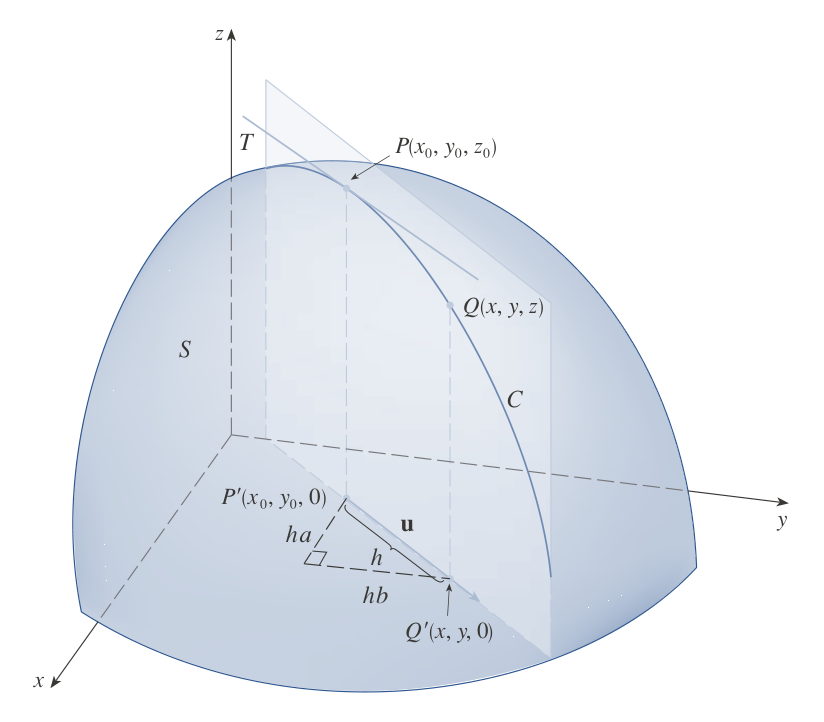
\includegraphics[width=0.6\linewidth]{imagenes/dv-direccional.png}
  \caption{Imagen sacada de \parencite{stewart2}.}
  \label{fig:dv-direccional}
\end{figure}

El plano vertical que pasa por $ P $ en la dirección $ \mathbf{u} $ interseca a $ S $ en un curva $ C $. La pendiente de la recta tangente $ T $ a $ C $ en el punto $ P $ es la razón de cambio de $ z $ en la dirección de $ \mathbf{u} $.

Si $ Q(x,y,z) $ es otro punto en $ C $ y $ P^{\prime}, Q^{\prime} $ son las proyecciones de $ P, Q $ en el plano $ xy $, el vector $ \vv{P^{\prime}Q^{\prime}} $ es paralelo a $ \mathbf{u} $ y por lo tanto
\[
\vv{P^{\prime}Q^{\prime}}=h\mathbf{u}=\left\langle ha,hb \right\rangle \qquad h \in \mathbb{R}^{}
\]

Así, $ x-x_{0}=ha $, $ y-y_{0}=hb $, entonces $ x=x_{0}+ha $ y $ y=y_{0}+hb $, con lo que podemos decir que
\[
	\frac{\Delta z}{h} = \frac{z-z_{0}}{h} = \frac{f(x_{0}+ha,y_{0}+hb)-f(x_{0},y_{0})}{h}
\]

Si calculamos el límite cuando $ h \to 0 $, obtenemos la razón de cambio de $ z $ en la dirección de $ \mathbf{u} $, que se conoce como \textbf{derivada direccional} de $ f $ en la dirección de $ \mathbf{u} $

\vspace{0.2cm}
\fbox{\parbox{0.9\linewidth}{
\textbf{Derivada direccional}

La derivada direccional de $ f $ en $ (x_{0},y_{0}) $ en la dirección de un vector unitario $ \mathbf{u}=\left\langle a,b \right\rangle $ es
\[
D_{u}f(x_{0},y_{0}) = \lim_{h \to 0}\frac{f(x_{0}+ha,y_{0}+hb)-f(x_{0},y_{0})}{h}
\]

si ese límite existe.
}}\vspace{0.2cm}

Viendo esta definición podemos ver que si $ \mathbf{u}=\mathbf{i}=\left\langle 1,0 \right\rangle $, entonces $ D_{i}f=f_{x} $, y que si $ \mathbf{u}=\mathbf{j}=\left\langle 0,1 \right\rangle $, entonces $ D_{j}=f_{y} $. Osea que, en realidad, las derivadas parciales respecto de $ y $ y $ x $ son casos especiales de las derivadas direccionales.

\vspace{0.2cm}
\fbox{\parbox{0.9\linewidth}{
\textbf{Teorema}

Si $ f $ es una función derivable de $ x $ y $ y $, entonces $ f $ tiene una derivada direccional en la dirección de cualquier vector unitario $ \mathbf{u}=\left\langle a,b \right\rangle $ y \[
D_{u}f(x,y)=f_{x}(x,y)a+f_{y}(x,y)b
\]
}}\vspace{0.2cm}

Tarea, demostrar ;)

\subsubsection{El vector gradiente}
Si vemos el teorema anterior, podemos notar que la derivada direccional de una función derivable puede escribirse comom el producto punto de dos vectores:
\begin{align*}
  D_{u}f(x,y) &= f_{x}(x,y)a+f_{y}(x,y)b\\
   &= \left\langle f_{x}(x,y),f_{y}(x,y) \right\rangle\cdot \left\langle a,b \right\rangle\\
  D_{u}f(x,y) &= \left\langle f_{x}(x,y),f_{y}(x,y) \right\rangle\cdot \mathbf{u}
\end{align*}

El primer vector en este producto recibe el nombre de \textbf{gradiente} de $ f $ y se denota como $ \nabla f $.

\vspace{0.2cm}
\fbox{\parbox{0.9\linewidth}{
\textbf{Gradiente}

Dada una función $ f:U \subset \mathbb{R}^{n} \to \mathbb{R}^{} $, podemos definir el gradiente de la función, y lo denotamos como $ \nabla f $, como un vector cuyas componentes son las derivadas parciales de todas sus variables independientes.
\[
\nabla f = \left\langle \pdv[]{f}{x_{1}},\pdv[]{f}{x_{2}},\dots ,\pdv[]{f}{x_{n}} \right\rangle
\]
}}\vspace{0.2cm}

Ademas, siempre podemos escribir la derivada direccional como el producto punto entre el vector gradiente y el vector unitario $ \mathbf{u} $ que marca la dirección.
\[
D_{u}f = \nabla f \cdot \mathbf{u}
\]

\subsubsection{Maximización de la derivada direccional}
Como la derivada direccional $ D_{u}f(x) $ es el producto escalar entre dos vectores $ \nabla f(x) \cdot \mathbf{\hat{u}} $, el \textbf{valor máximo} de la derivada direccional lo vamos a obtener cuando la dirección de $ \nabla f(x) $ sea la misma que el versor $ \mathbf{\hat{u}} $. Esto es porque cuando dichos vectores tienen la misma dirección el producto escalar dá su valor máximo ya que el $ \cos^{}(\theta)=1 $. Cuando esto ocurre, el valor de la derivada direccional $ D_{u}f(x) = \lVert\nabla f(x)\rVert $.

\underline{Ejemplo:}

\begin{enumerate}[a)]
  \item Si $ f(x,y)=xe^y $, determine la razón de cambio de $ f $ en el punto $ P(2,0) $ en la dirección de $ P  \to Q(\frac{1}{2},2) $.

  \item ¿En qué dirección tiene $ f $ la máxima razón de cambio? ¿Cuál es la máxima razón de cambio?
\end{enumerate}

\begin{enumerate}[a)]
	\item Nos piden obtener la derivada direccional de $ f(x,y)=xe^y $ en el punto $ P(2,0) $, en dirección $ P \to Q(\frac{1}{2},2) $.
		\[
			D_{\vv{PQ}}f(x,y) = \nabla f(x,y) \cdot \frac{\vv{PQ}}{\lVert\vv{PQ}\rVert}
		\]
		\[
			\nabla f(x,y) = \left\langle f_{x},f_{y} \right\rangle = \left\langle e^y,xe^y \right\rangle
		\]
		
	El versor en la dirección $ \vv{PQ}=\left\langle -\frac{3}{2} \right\rangle $ es $ \mathbf{\hat{u}}=\left\langle -\frac{3}{5},\frac{4}{5} \right\rangle $, así que la razón de cambio de $ f $ en la diarección $ \vv{PQ} $ es
	\[
	D_{u}f(2,0)=\nabla f(2,0)\cdot \mathbf{\hat{u}} = \left\langle 1,2 \right\rangle \cdot \left\langle -\frac{3}{5},\frac{4}{5} \right\rangle = 1
	\]

\item La máxima razón de cambio se dá cuando $ \mathbf{\hat{u}} $ tiene la misma dirección de $ \nabla f(x,y) $, y es igual a $ \lVert\nabla f(x,y)\rVert $ en el punto $ (2,0) $
	\[
	\lVert\nabla f(2,0)\rVert = \lVert\left\langle 1,2 \right\rangle\rVert = \sqrt[]{5}
	\]
\end{enumerate}

\subsection{Planos tangentes a superficies}
Supongamos que $ S $ es una superficie de nivel con ecuación $ F(x,y,z)=k $, y sea $ P(x_{0},y_{0},z_{0}) $ un punto en $ S $. Sea $ C $ \textit{cualquier} curva de la superficie $ S $ que pasa por el punto $ P $. La función de la curva que pasa $ C $ la podemos escribir en su forma paramétrica de manera que $ C = r(t) = \left\langle x(t),y(t),z(t) \right\rangle $. Sea $ t_{0} $ el valor paramétrico correspondiente a $ P $; es decir, $ r(t_{0}) = \left\langle x_{0},y_{0},z_{0} \right\rangle $. Como $ C $ reside en $ S $, cualquier punto $ \left(x(t),y(t),z(t)\right) $, debe satisfacer la ecuación de $ S $, es decir
\begin{equation}\label{eq:sup-nivel}
F\left(x(t),y(t),z(t)\right) = k
\end{equation}

Si en la ecuación \ref{eq:sup-nivel}, $ x $, $ y $ y $ z $ son funciones derivables de $ t $ y $ F $ también es derivable, podemos derivar $ F $ respecto de $ t $ usando la regla de la cadena como sigue:
\begin{equation}\label{eq:dv-sup-nivel-Ft}
\pdv[]{F}{x}\dv[]{x}{t} + \pdv[]{F}{y}\dv[]{y}{t} + \pdv[]{F}{z}\dv[]{z}{t} = 0
\end{equation}

Pero habíamos visto que $ \nabla F = \left\langle F_{x}, F_{y}, F_{z} \right\rangle $ y sabemos que $ r^{\prime}(t)=\left\langle x^{\prime}(t),y^{\prime}(t),z^{\prime}(t) \right\rangle $, así que a la ecuación \ref{eq:dv-sup-nivel-Ft} la podemos expresar como un producto punto de la siguiente forma
\[
  \left\langle F_{x},F_{y},F_{z} \right\rangle\cdot \left\langle \dv[]{x}{t},\dv[]{y}{t},\dv[]{z}{t} \right\rangle = 0
\]
\begin{equation}\label{eq:grad-plano-tg}
  \nabla F\cdot r^{\prime}(t)=0
\end{equation}

Si lo analizamos cuando $ t = t_{0} $ tenemos que $ r(t_{0})=\left\langle x_{0},y_{0},z_{0} \right\rangle $, así que
\begin{equation}\label{eq:plano-tg-punto}
  \nabla F(x_{0},y_{0},z_{0})\cdot r^{\prime}(t_{0})=0
\end{equation}

La ecuación \ref{eq:plano-tg-punto} establece que \textit{el vector gradiente en $ P $ dado por $ \nabla F(x_{0},y_{0},z_{0}) $, es perpendicular al vector tangente $ r^{\prime}(t_{0}) $ a cualquier curva $ C $ en $ S $ que pase por $ P $}. De esta manera podemos afirmar que, si $ \nabla F(x_{0},y_{0},z_{0})\neq 0 $, el \textbf{plano tangente a la superficie de nivel} $ F(x,y,z) = k $ en el punto $ P(x_{0},y_{0},z_{0}) $ es el plano cuyo vector normal es $ \nabla F(x_{0},y_{0},z_{0}) $ y pasa por el punto $ P $.

La ecuación del \textbf{plano tangente a la superficie de nivel} $ F(x,y,z) = k $ está dada por la ecuación \ref{eq:plano-tg-punto}

En el caso especial enel que la ecuación de una superficie $ S $ es de la forma $ z=f(x,y) $, podemos definir la ecuación como
\[
  F(x,y,z) = f(x,y) - z = 0
\]

y considerar a $ S $ como una superficie de nivel con $ k=0 $, de manera que
\begin{align*}
  F_{x}(x_{0},y_{0},z_{0}) &= f_{x}(x_{0},y_{0})\\
  F_{y}(x_{0},y_{0},z_{0}) &= f_{y}(x_{0},y_{0})\\
  F_{z}(x_{0},y_{0},z_{0}) &= -1
\end{align*}

\subsection{Máximos y mínimos}
\vspace{0.2cm}
\fbox{\parbox{0.9\linewidth}{
\textbf{Definición}

Una función de dos variables tiene un \textbf{máximo local} en $ (a,b) $ si $ f(x,y) \leq f(a,b) $ cuando $ (x,y) $ está cerca de $ (a,b) $. El número $ f(a,b) $ se llama \textbf{valor máximo local}. 

Si $ f(x,y) \geq f(a,b) $ cuando $ (x,y) $ está cerca de $ (a,b) $, $ f $ tiene un \textbf{mínimo local} en $ (a,b) $ y $ f(a,b) $ es un \textbf{valor mínimo local}
}}\vspace{0.2cm}

Si las desigualdades de la definición anterior son válidas para todos los puntos $ (x,y) $ en el dominio de $ f $, entonces $ f $ tiene un \textbf{máximo absoluto} (o \textbf{mínimo absoluto}) en $ (a,b) $.

Si $ f $ tiene un máximo o mínimo local en $ (a,b) $ y las derivadas parciales existen, entonces $ f_{x}(a,b)=0 $ y $ f_{y}(a,b)=0 $. En otras palabras, si hay un máximo o un mínimo en $ (a,b) $, el gradiente de $ f $ es cero $ \nabla f(a,b)=0 $.

Un \textbf{punto crítico} de $ f $ es cuando $ f_{x}(a,b)=0 $ o $ f_{y}(a,b)=0 $ o si una de las derivadas parciales no existe. Todos los máximos y mínimos de $ f $ son puntos críticos, pero no todos los puntos críticos son máximos y mínimos de $ f $.

\underline{Ejemplo:} Sea $ f(x,y)=x^2 + y^2 - 2x-6y+14 $. Entonces,
\begin{align*}
	f_{x}(x,y) = 2x-2 && f_{y}(x,y)=2y-6
\end{align*}
Estas derivadas parciales son iguales a cero cuando $ x=1 $ y $ y=3 $, así que el único punto crítico es $ (1,3) $. 

Generalmente conviene completar los cuadrados para facilitar los cálculos, la función entonces nos quedaría así:
\begin{align*}
  f(x,y) &= (x-1)^2 + (y-3)^2 + 4
\end{align*}
Al evaluar la función en el punto $ (1, y) $ nos queda $ (y-3)^2 \geq 0 $, y cuando evaluamos la función en el punto $ (x,3) $ obtenemos $ (x-1)^2 \geq 0 $. Esto nos dice que la función crece en la dirección de $ x $ y también en la dirección de $ y $ a partir del punto $ (1,3) $, por lo que si reemplazamos $ (x,y) $ por el punto crítico $ (1,3) $ en la ecuación, nos dá 4, que es un mínimo local. De hecho, como el vértice del paraboloide se encuentra en el punto $ (1,3,4) $, la función SIEMPRE va a ser mayor a o igual 4, así que $ f(1,3)=4 $ es un mínimo absoluto de $ f $.

\begin{center}
\begin{tikzpicture}
  \begin{axis}[
    title={$ f(x,y)=(x-1)^2+(y-3)^2+4 $},
    xlabel=$x$, ylabel=$y$, zlabel={$f(x,y)$},
    view={120}{10},
    xmin=0, xmax=6,
    ymin=0, ymax=6,
    zmin=0, zmax=15,
    point meta min=4, point meta max=15,
    axis lines=center,
    axis on top=true,
    samples=40,
  ]
    \addplot3 [surf, shader=flat,  colormap/viridis,]
	    {(x-1)^2 + (y-3)^2 + 4};
    \addplot3[only marks, mark=*,mark size=5pt,color=red,]
	    coordinates {(1,3,4)};
    \node at (axis cs:1,3,4) [anchor=north] {$P(1,3,4)$};
  \end{axis}
\end{tikzpicture}
\end{center}

\underline{Ejemplo 2:} Sea $ f(x,y)=y^2-x^2 $. Entonces,
\begin{align*}
	f_{x}(x,y) = -2x && f_{y}(x,y)  = 2y
\end{align*}

Las derivadas se hacen cero cuando $ x = y = 0 $, así que tenemos un solo punto crítico en el $ (0,0) $. Sin embargo, cuando ahora analizamos la función para cada uno de los puntos vemos que a veces crece, y otras decrece: $ f(0,y)=y^2 \geq 0 $, pero $ f(x,0)=-x^2 \leq 0 $. En consecuencia, todos los discos con centro $ (0,0) $ contienen puntos donde $ f $ adopta valores positivos, así como puntos en los que $ f $ adopta valores neagtivos. Por lo tanto, $ f(0,0)=0 $ no puede ser ni un mínimo ni un máximo de $ f $. Es un \textbf{punto silla}.

\begin{center}
\begin{tikzpicture}
  \begin{axis}[
	  title={$ f(x,y)=y^2-x^2 $},
	  xlabel=$x$, ylabel=$y$, zlabel={$f(x,y)$},
	  view={110}{20},
	  axis lines=center,
	  axis on top=true,
	  ]
    \addplot3 [surf, shader=flat, colormap/viridis,]
	    {y^2-x^2};
    \addplot3 [only marks, mark=*, mark size=5pt, color=red]
	    coordinates{(0,0,0)};
  \end{axis}
\end{tikzpicture}
\end{center}

Podemos ver entonces que no alcanza solo con calcular los puntos críticos de una función para determinar si esta tiene máximos o mínimos. Existen distintos métodos para determinarlo pero el mas común es el de calcular la determinante del \textbf{Hessiano}. El \textbf{Hessiano} es la matriz compuesta con las segundas derivadas de la función $ f $.

\vspace{0.2cm}
\fbox{\parbox{0.9\linewidth}{
\textbf{Prueba de la segunda derivada}

Si la función $ f(x,y) $ tiene un punto crítico en $ (a,b) $ (osea que $ f_{x}(a,b)=0 $ y $ f_{y}(a,b)=0 $), y las segundas derivadas de $ f $ son continuas en un disco con centro en $ (a,b) $, entonces podemos armar el \textbf{Hessiano} ($ H_{f} $) y calcular su determinante ($ \det(H_{f}) $) para determinar los extremos (mínimos, máximos y/o puntos silla) de $ f $.
\begin{enumerate}[a)]
  \item Si $ \det(H_{f}) > 0 $ y $ f_{xx}(a,b)>0 $, entonces $ f(a,b) $ es un mínimo local.

  \item Si $ \det(H_{f})>0 $ y $ f_{xx}(a,b)<0 $, entonces $ f(a,b) $ es un máximo local.

  \item Si $ \det(H_{f})<0 $, entonces $ f(a,b) $ es un punto silla.

  \item Si $ \det(H_{f})=0 $, entonces este método no sirve y no aporta información útil.
\end{enumerate}
}}\vspace{0.2cm}

\underline{Ejemplo 3:} Encontrar los valores máximos y mínimos locales, y los puntos silla de la función $ f(x,y)=x^4+y^4-4xy+1 $.

Lo primero que hacemos es encontrar los puntos críticos:
\begin{align*}
  f_{x} = 4x^3-4y && f_{y}=4y^3-4x
\end{align*}

Al igualar a cero las derivadas parciales se obtiene el siguiente sistema de ecuaciones:
\[
\begin{cases}
  4(x^3-y) = 0\\
  4(y^3-x) = 0
\end{cases} \implies \begin{cases}
  x^3=y\\
  y^3=x 
\end{cases} \implies (x^3)^3 - x = 0  
\]
\[
  \implies 0=x(x^8-1)=x(x^4-1)(x^4+1)=x(x^2-1)(x^2+1)(x^4+1)
\]

De manera que hay tres raíces reales: $ x=\left\{0,1,-1\right\} $. Los tres puntos críticos son $ (0,0) $, $ (1,1) $ y $ (-1,-1) $.

Ahora calculamos las segundas derivadas para poder armar el Hessiano:
\begin{align*}
  f_{xx} = 12x^2 && f_{xy} = -4 && f_{yx} = -4 && f_{yy} = 12y^2
\end{align*}

El Hessiano y su determinante nos quedan así:
\[H_{f}=
  \begin{bmatrix}
	  12x^2 & -4 \\
	  -4 & 12y^2
  \end{bmatrix} \quad  , \quad 
 \det(H_{f}) = 144x^2y^2-16 
\]

Al analizar la $ \det(H_{f}) $ en el punto $ (0,0) $ obtenemos $ \det(H_{f}(0,0))=-16 < 0 $, que por el caso (c) de la prueba de la segunda derivada sabemos que es un punto silla.

Si calculamos la determinante en el punto $ (1,1) $ obtenemos $ \det(H_{f}(1,1))=128>0 $, y $ f_{xx}(1,1)=12>0 $, así que estamos en el caso (a) que nos dice que $ f(1,1)=-1 $ es un mínimo local. Lo mismo pasa cuando calculamos la determinante en el punto $ (-1,-1) $ que nos da $ \det(H_{f}(-1,-1))=128>0 $ y $ f_{xx}(-1,-1)=12>0 $, así que $ f(-1,-1)=-1 $ también es un mínimo local.


\begin{center}
\begin{tikzpicture}
  \begin{axis}[
    title={$f(x,y)=x^4+y^4-4xy+2$},
    xlabel={$x$}, ylabel={$y$}, zlabel={$f(x,y)$},
    view={100}{20},
    axis lines=center,
    axis on top=true,
    domain=-2:2, y domain=-2:2,
    xmin=-2, xmax=2,
    ymin=-2, ymax=2,
    zmax=5, point meta max=5,
    samples=60,
  ]
  \addplot3 [surf, shader=flat, colormap/viridis,]
	  {pow(x,4)+pow(y,4)-4*x*y+2};
  \addplot3 [only marks, mark=*, mark size=5pt, color=red,]
    coordinates{(0,0,2)};
  \node at (axis cs:0,0,2) [anchor=north] {$P(0,0,2)$};
  \addplot3 [only marks, mark=*, mark size=5pt, color=red,]
    coordinates{(1,1,0)};
  \node at (axis cs:1,1,0) [anchor=north] {$P(1,1,0)$};
  \addplot3 [only marks, mark=*, mark size=5pt, color=red,]
    coordinates{(-1,-1,0)};
  \node at (axis cs:-1,-1,0) [anchor=north] {$P(-1,-1,0)$};
  \end{axis}
\end{tikzpicture}
\end{center}

\underline{Ejemplo 4:} Una caja rectangular sin tapa debe hacerse con $ 12 m^2 $ de cartón. Determine el volumen máximo de esa caja.

Podemos decir que la caja va a tener un largo $ x $, ancho $ y $, y alto $ z $. Entonces el volumen de la caja es:
\[
  V=xyz
\]

Este volumen $ V $ lo podemos expresar como una función de solo dos variables $ x $ y $ y $ si podemos escribir a $ z $ en función de $ (x,y) $. Para eso lo que podemos hacer es buscar cuál es el área de de las caras de la caja que tenemos que armar y despejar $ z $ de ahí.

Los datos que tenemos son que contamos con $ 12m^2 $ de cartón, con los que tenemos que armar una caja rectangular sin tapa. Osea que con esos $ 12m^2 $ tenemos que poder armar las cinco caras de la caja (no son seis porque no tiene tapa). 

\begin{center}
\begin{tikzpicture} % coordenadas son (y,z,x)
\newcommand{\ancho}{3}
\newcommand{\alto}{3}
\newcommand{\largo}{5}
\coordinate (O) at (0,0,0);
\coordinate (A) at (0,0,\ancho);
\coordinate (B) at (0,\alto,\ancho);
\coordinate (C) at (\largo,\alto,\ancho);
\coordinate (D) at (\largo,0,\ancho);
\coordinate (E) at (0,\alto,0);
\coordinate (F) at (\largo,\alto,0);
\coordinate (G) at (\largo,0,0);

\fill [blue!30] (O) -- (A) -- (D) -- (G) -- cycle;	% abajo
\fill [blue!30] (O) -- (E) -- (F) -- (G) -- cycle;	% atras
\fill [blue!30] (O) -- (A) -- (B) -- (E) -- cycle;	% atras
\fill [blue!50] (D) -- (G) -- (F) -- (C) -- cycle;	% adelante
\fill [blue!50] (A) -- (B) -- (C) -- (D) -- cycle;	% derecha

\draw   (D) edge[below, ] node{$ x $} (G)
	(A) edge[below, ] node{$ y $} (D)
	(A) edge[left, ] node{$ z $} (B)
	(D) edge[, ] node{} (C)
	(G) edge[, ] node{} (F)
	(O) edge[dashed ] node{} (G)
	(O) edge[dashed, ] node{} (A)
	(O) edge[dashed, ] node{} (E)
;
\end{tikzpicture}
\end{center}

La suma del area de las 5 caras nos tiene que dar los $ 12m^2 $ de los que disponemos. Tenemos entonces dos caras que podemos calcular su área como $ xz $, dos caras cuya área es $ zy $ y una cara que es la de abajo $ xy $. Entonces la ecuación nos queda así:
\[
  12 = 2xz + 2zy + xy
\]

Ahora podemos despejar $ z $ de la ecuación:
\begin{align*}
  2xz + 2zy + xy &= 12\\
  2z(x+y)+xy &= 12\\
  \frac{12-xy}{2(x+y)} &= z
\end{align*}

Y con esto, podemos reemplazar $ z $ en la ecuación del volumen $ V $:
\[
	V = xy\left(\frac{12-xy}{2(x+y)}\right) = \frac{12xy-x^2y^2}{2(x+y)}
\]

Y ahora que ya tenemos nuestra función de dos variables, solo queda realizar los pasos anteriores y determinar los extremos de la función. Como estamos buscando la caja que tenga el volumen máximo, tenemos que buscar valores máximos de la función.

Calculamos las derivadas parciales:
\begin{align*}
  \pdv[]{V}{x} = \frac{y^2(12-2xy-x^2)}{2(x+y)^2} && \pdv[]{V}{y} = \frac{x^2(12-2xy-y^2)}{2(x+y)^2}
\end{align*}

Igualamos a creo las derivadas parciales y resolvemos el sistema de ecuaciones:
\[
\left\{
\begin{aligned}
  \pdv[]{V}{x} = \frac{y^2(12-2xy-x^2)}{2(x+y)^2} = 0 \\
  \pdv[]{V}{y} = \frac{x^2(12-2xy-y^2)}{2(x+y)^2} = 0
\end{aligned}
\right.
\]  

Vemos que parece que hay un punto crítico en el punto $ (0,0) $ pero en realidad no es así ya que en ese punto la ecuación no es derivable (el denominador se hace cero). Así que hay que resolver el sistema normalmente:
\[
  \left\{
  \begin{aligned}
    12-2xy-x^2 = 0 \\
    12-2xy-y^2 = 0
  \end{aligned}
  \right.  \implies x^2 = y^2  \implies x = y
\]

Si reemplazamos cualquier ecuación con $ x = y $ obtenemos $ 12 - 3x^2 = 0 $, que nos da $ x = \pm 2 $, o si reemplazamos con $ y=x $, $ y=\pm 2 $. De esta manera sabemos que hay puntos críticos en $ (2,2) $ y $ (-2,-2) $.

El siguiente paso sería calcular $ H_{f} $ y evaluar su determinante en los puntos críticos, pero en este caso esa matríz es dificil de calcular. Lo que sí podemos hacer es analizar el problema y pensarlo logicamente: sabemos que el volumen máximo se va a encontrar en alguno de los puntos críticos. Tenemos los $ x $ y $ y $ de los puntos críticos, pero para calcular el volumen necesitamos conocer el valor de $ z $ también. Esto lo podemos hacer facil reemplazando los valores del punto crítico en la ecuación que habíamos encontrado para $ z $ un poco mas arriba. Entonces, para $ (2,2) $ tenemos:
\[
  z = \frac{12-2 \cdot  2}{2(2+2)} = 1
\]

, nos queda entonces el punto $ (2,2,1) $. Y para el punto $ (-2,-2) $ tenemos:
\[
  z = \frac{12-(-2)\cdot (-2)}{2((-2)+(-2))} = -1
\]

, quedándonos el punto $ (-2,-2,-1) $. 

Vayamos ahora a calcular el volumen en los dos puntos obtenidos y fijémonos cuál es el máximo.
Para $ (2,2,1) $ tenemos:
\[
  V = 2\cdot 2\cdot 1 = 4
\]

Para $ (-2,-2,-1) $ tenemos:
\[
  V = (-2)\cdot (-2) \cdot (-1) = -4
\]

Un volumen negativo no tiene sentido, así que el volumen máximo de la caja que se puede alcanzar con $ 12m^2 $ de cartón es $ 4m^3 $.

\subsection{Valores máximos y mínimos absolutos}
Para una función $ f $ de una variable, el teorema de los valores extremos establece que si $ f $ es continua en un intervalo cerra $ \left[a,b\right] $, $ f $ tiene un valor mínimo absoluto y valor máximo absoluto. Esos valores se determinan evaluando $ f $ no solo en los números críticos, sino también en los puntos extremos $ a $ y $ b $. 

Lo mismo que pasaba para las funciones escalares, pasa para las funciones de varias variables.

\vspace{0.2cm}
\fbox{\parbox{0.9\linewidth}{
\textbf{Teorema de los valores extremos para funciones de dos variables}

Si $ f $ es continua en un conjunto cerrado y acotado $ D $ en $ \mathbb{R}^{2} $, entonces $ f $ alcanza un valor máximo absoluto $ f(x_{1},y_{1}) $ y un valor mínimo absoluto $ f(x_{2},y_{2}) $ en algunos puntos en $ D $.
}}\vspace{0.2cm}

De esta manera, podemos extender el teorema de los valores extremos relativos

\vspace{0.2cm}
\fbox{\parbox{0.9\linewidth}{
\textbf{}

Para determinar los valores máximo y mínimo absolutos de una función continua $ f $ en un conjunto cerrado y acotado $ D $:
\begin{enumerate}[1.]
  \item Determinamos los valores de $ f $ en los puntos críticos de en $ f $ en $ D $.

  \item Determinamos los valores extremos de $ f $ en la frontera de $ D $.

  \item El mayor de los valores de los pasos 1 y 2 es el valor máximo absoluto; el menor de esos valores es el mínimo absoluto.
\end{enumerate}
}}\vspace{0.2cm}

\underline{Ejemplo:} Hallar los valores máximo y mínimo absoluto de la función $ f(x,y)=x^2-2xy+2y $ en el rectángulo $ D=\left\{(x,y) \;/\; 0 \leq x \leq 3  \land 0 \leq y \leq 2\right\} $.

Sabemos que $ f $ es continua en el rectángulo cerrado y acotado $ D $ porque es una función polinómica. Lo primero que hacemos entonces es determinar los puntos críticos:
\begin{align*}
  f_{x}=2x-2y = 0 && f_{y}=-2x+2 = 0
\end{align*}

El único punto crítico es $ (1,1) $, y el valor de $ f $ ahí es $ f(1,1)=1 $.

El siguiente paso es determinar los valores extremos de $ f $ en la frontera de $ D $, que en este caso son los cuatro segmentos de recta $ L_{1},L_{2},L_{3},L_{4} $ que delimitan el cuadrado $ D $.

\begin{center}
\begin{tikzpicture}
  \begin{axis}[
    width=8cm, % height=9cm,
    %every axis/.append style={font=\Large},
    axis lines=center,
    xtick={0,...,3},
    ytick={0,...,2},
    xmin=-0.5, xmax=3.5,
    ymin=-0.5, ymax=2.5,
  ]
     \addplot [domain=0:3, blue]{2}
	     node[above, pos=0.5]{$ L_{3} $};
     \addplot [domain=0:3, blue]{0}
	     node[above, pos=0.5]{$ L_{1} $};
     \addplot [domain=0:2, blue]({3},x)
	     node[right, pos=0.5]{$ L_{2} $};
     \addplot [domain=0:2, blue]({0},x)
	     node[right, pos=0.5]{$ L_{4} $};
  \end{axis}
\end{tikzpicture}
\end{center}

El segmento $ L_{1} $ está dado por la ecuación $ L_{1}:y=0  \land 0\leq x\leq 3 $. Si evaluamos la recta $ L_{1} $ en la ecuación $ f $ obtenemos:
\[
  f(x,0)=x^2 \qquad 0\leq x\leq 3
\]
el valor mínimo de esta función es $ f(0,0)=0 $ y el máximo es $ f(3,0)=9 $.

Para $ L_{2} $ tenemos que:
\[
  f(3,y)=9-4y \qquad 0\leq y\leq 2
\]
el valor máximo es $ f(3,0)=9 $ y su valor mínimo es $ f(3,2)=1 $.

Para $ L_{3} $ tenemos:
\[
  f(x,2)=x^2-4x+4 \qquad 0\leq x\leq 3
\]
el valor mínimo de esta función es $ f(2,2)=0 $ y el valor máximo es $ f(0,2)=4 $. 

Por último, para $ L_{4} $ tenemos:
\[
  f(0,y)=2y \qquad 0\leq y\leq 2
\]
que tiene valor mínimo $ f(0,0)=0 $ y valor máximo $ f(0,2)=4 $. 

De esta manera, determinamos que el valor máximo en la frontera es 9 y el valor mínimo en la misma es 0.

En el paso 3 tenemos que comparar los valores de la función evaluada en la frontera contra los valores de la función en los puntos críticos. Y ahora sí podemos concluir que el valor máximo absoluto de $ f $ en $ D $ es $ f(3,0)=9 $ y el valor mínimo absoluto es $ f(0,0)=f(2,2)=0 $.

\begin{center}
\begin{tikzpicture}
  \begin{axis}[
    title={$f(x,y)=x^2-2xy+2y$},
    clip=false,
    xlabel={$x$}, ylabel={$y$}, zlabel={$f(x,y)$},
    view={110}{20},
    axis lines=center,
    %axis on top=true,
    domain=0:3, y domain=0:2,
    zmax=9, point meta max=9,
  ]
  \addplot3 [surf, shader=flat, colormap/viridis, ]
    {x^2-2*x*y+2*y};
  \addplot3 [only marks, mark=*, mark size=5pt, color=red,]
    coordinates{(0,0,0)};
  \node at (axis cs:0,0,0) [anchor=south] {$P(0,0,0)$};
  \addplot3 [only marks, mark=*, mark size=5pt, color=red,]
    coordinates{(2,2,0)};
  \node at (axis cs:2,2,0) [anchor=north] {$P(2,2,0)$};
  \addplot3 [only marks, mark=*, mark size=5pt, color=red,]
    coordinates{(3,0,9)};
  \node at (axis cs:3,0,9) [anchor=north] {$P(3,0,9)$};
  \end{axis}
\end{tikzpicture}
\end{center}

\subsection{Multiplicadores de Lagrange}
Hace un rato habíamos resuelto un ejercicio en el que teníamos que maximizar una función de volumen $ V = xyz $ que estaba sujeta a una restricción $ 2xz + 2yz + xy = 12 $, que representaba la condición secundaria de que el área del cartón que teníamos para armar la caja era de $ 12m^2 $. Este tipo de operaciones, en las que buscamos maximizar o minimizar una función general $ f(x,y,z) $ (en nuestro caso era la función del volumen) sujeta a una restricción de la forma $ g(x,y,z)=k $ (en nuestro caso era la función del área=12) es mucho mas fácil resolverlas usando el método de Lagrange.

Este método conviene primero analizarlo para funciones de dos variables y una vez que lo entendemos geométricamente podemos estudiarlo para funciones de tres variables. Entonces, supongamos que tenemos una función $ f(x,y) $ y queremos encontrar los valores extremos cuando el punto $ (x,y) $ está restringido a residir en la curva de nivel $ g(x,y)=k $. 

\begin{figure}[H]
  \centering
  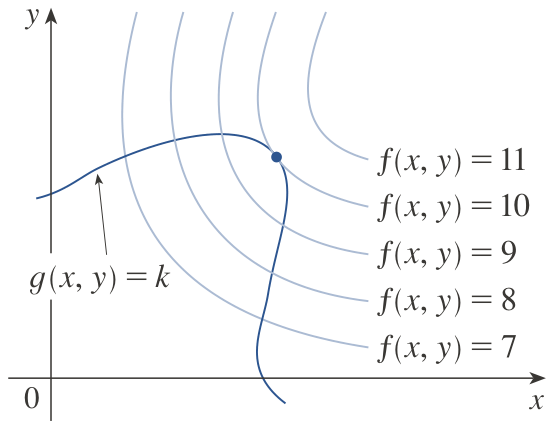
\includegraphics[width=0.4\linewidth]{imagenes/lagrange_2_variables.png}
  \caption{Imagen sacada de \parencite{stewart2}. Extremos de una función $ f $ restringida a la curva de nivel $ g(x,y)=k $.}
  \label{fig:lagrange}
\end{figure}

En la Figura \ref{fig:lagrange} podemos ver la curva $ g(x,y)=k $ y varias curvas de nivel de $ f $, dadas por $ f(x,y)=c $ donde $ c= 7,8,9,10,11 $. Maximizar $ f(x,y) $ sujeta a $ g(x,y)=k $ consiste en encontrar el mayor valor de $ c $ tal que la curva $ f(x,y)=c $ interseque $ g(x,y)=k $. Podemos ver que esto sucede cuando dichas curvas apenas se tocan, osea, cuando tienen una recta tangente común. Esto significa que las rectas normales a cada curva en el punto $ (x_{0},y_{0}) $ donde se tocan son indénticas. Lo que quiere decir que los vectores gradiente son paralelos; es decir, $ \nabla f(x_{0},y_{0}) = \lambda \nabla g(x_{0},y_{0}) $ con $ \lambda  \in \mathbb{R}^{} $.

El mismo argumento aplica cuando queremos encontrar valores extremos de $ f(x,y,z) $ sujeta a la restricción $ g(x,y,z)=k $, solo ahora en vez de pensar en curvas de nivel tenemos que pensar en superficies de nivel. Como los vectores gradiente de $ f $ y $ g $ son paralelos, podemos decir que si $ \nabla g(x_{0},y_{0},z_{0})\neq \vv{0} $, existe un $ \lambda  \in \mathbb{R}^{} $ tal que
\[
  \nabla f(x_{0},y_{0},z_{0}) = \lambda \nabla g(x_{0},y_{0},z_{0})
\]

El número $ \lambda $ se llama \textbf{multiplicador de Lagrange}.

\vspace{0.2cm}
\fbox{\parbox{0.9\linewidth}{
\textbf{Método de multiplicadores de Lagrange}

Para determinar los valores máximo y mínimo de $ f(x,y,z) $ sujetos a la restricción $ g(x,y,z)=k $ (suponiendo que esos valores existen y que $ \nabla g \neq \vv{0} $ en la superficie $ g(x,y,z)=k $):
\begin{enumerate}[1.]
  \item Determinamos todos los valores de $ x $, $ y $, $ z $ y $ \lambda $ tales que
	  \[
	    \nabla f(x,y,z)=\lambda \nabla g(x,y,z)
	  \]
	  y
	  \[
	    g(x,y,z)=k
	  \]

  \item Evaluamos $ f $ en todos los puntos $ (x,y,z) $ que resulten del paso (1). El mayor de esos valores es el valor máximo de $ f $; el menor es el valor mínimo de $ f $.
\end{enumerate}
}}\vspace{0.2cm}

Cuando escribamos la ecuación $ \nabla f = \lambda \nabla g $ vamos a tener un sistema de cuatro ecuaciones con cuatro incógnitas
\[
  \left\{
  \begin{aligned}
	  f_{x} &= \lambda g_{x} \\
	  f_{y} &= \lambda g_{y} \\
	  f_{z} &= \lambda g_{z} \\
	  g(x,y,z) &= k
  \end{aligned}
  \right.
\]
pero no es necesario encontrar valores para $ \lambda $.


\underline{Ejemplo:} Se quiere armar una caja rectangular sin tapa con $ 12m^2 $ de cartón. Determine el volumen máximo de esa caja.

Este es el mismo ejemplo que habíamos hecho antes, solo que ahora lo vamos a resolver usando el método de los multiplicadores de Lagrange. Igual que hicimos antes, vamos a definir $ x $, $ y $ y $ z $ como la longitud, ancho y alto de la caja. Así que la función que queremos maximizar es:
\[
  V=xyz
\]
sujeta a la restricción
\[
  g(x,y,z)=2xz+2yz+xy=12
\]

Lo que tenemos que hacer es buscar los valores de $ x $, $ y $, $ z $ y $ \lambda $ tales que $ \nabla V = \lambda \nabla g $ y $ g(x,y,z)=12 $. Tenemos entonces el siguiente sistema de ecuaciones:
\[
  \left\{
  \begin{aligned}
	  V_{x} &= \lambda g_{x} \\
	  V_{y} &= \lambda g_{y} \\
	  V_{z} &= \lambda g_{z} \\
	  12 &=2xz + 2yz + xy 
  \end{aligned}
  \right. \implies \left\{
  \begin{aligned}
	  yz &= \lambda \left(2z+y\right) & (1)\\
	  xz &= \lambda \left(2z+x\right) & (2)\\
	  xy &= \lambda \left(2x+2y\right) & (3)\\
	  12 &=2xz + 2yz + xy & (4)\\
  \end{aligned}
  \right.
\]

Y ahora hay que ingeniarselas y resolver el sistema.

Lo primero que vemos es que $ \lambda $ no puede ser cero porque implicaría que $ yz=xz=xy $ y esto es imposible por la última ecuación. Por otro lado, podemos multiplicar (1) por $ x $, (2) por $ y $ y (3) por $ z $ y vemos que nos quedan los tres lados izquierdos de la ecuación todos iguales.
\[
  \left\{
  \begin{aligned}
	  xyz &= \lambda \left(2xz+xy\right) & (5)\\
	  yxz &= \lambda \left(2yz+yx\right) & (6)\\
	  zxy &= \lambda \left(2zx+2zy\right) & (7)\\
	  12 &=2xz + 2yz + xy & (4)
  \end{aligned}
  \right.
\]

De (6) y (7) podemos decir que 
\[
  2xz + xy = 2yz + xy
\]
que nos dice que $ xz=yz $. Pero $ z\neq 0 $ porque el volúmen de la caja no puede ser cero, así que $ x=y $. De (7) y (8) tenemos que
\[
  2yz + xy = 2xz + 2yz
\]
de donde sale que $ xy=2xz $, y por lo tanto $ y=2z $ ya que $ x\neq 0 $. Y ya resolvimos nuestro sistema de ecuaciones. Ahora podemos poner $ x=y=2z $ en (4) y obtenemos
\[
  4z^2+4z^2+4z^2 = 12
\]

Como $ x $, $ y $ y $ z $ son positivas (porque no podemos tener volumen o áreas negativas), se tiene que $ z=1 $, así que $ x=y=2 $. Y esta respuesta es la misma a la que habíamos llegado antes.

\underline{Ejemplo 2:} Determinar los valores extremos de la función $ f(x,y)=x^2+2y^2 $ en el círculo $ x^2+y^2=1 $

Usando el método de Lagrange resolvemos el sistema $ \nabla f = \lambda \nabla g $.
\[
  \left\{
  \begin{aligned}
	  2x &= \lambda 2x & (1) \\
	  4y &= \lambda 2y & (2) \\
	  1 &= x^2 + y^2 & (3)
  \end{aligned}
  \right.
\]

De (1) sabemos que $ x=0 $ o $ \lambda = 1 $. Si $ x=0 $, entonces (3) da $ y=\pm 1 $. Si $ \lambda = 1 $, entonces $ y=0 $ por la ecuación (2), así que (3) da $ x=\pm1 $. Por lo tanto, $ f $ tiene posibles valores extremos en los puntos $ (0,1) $, $ (0,-1) $, $ (1,0) $ y $ (-1,0) $. Si evaluamos $ f $ en dichos puntos tenemos 
\begin{align*}
  f(0,1) = 2 & f(0,-1)=2 & f(1,0)=1 & f(-1,0) = 1
\end{align*}

De manera que el valor máximo de $ f $ en el círculo $ x^2+y^2=1 $ es $ f(0,\pm1)=2 $ y el valor mínimo es $ f(\pm1,0)=1 $

\underline{Ejemplo 3:} Hallar los puntos en la esfera $ x^2+y^2+z^2=4 $ que están mas cerca y mas lejos del punto $ (3,1,-1) $.

La distancia desde un punto $ (x,y,z) $ al punto $ (3,1,-1) $ es 
\[
  d=\sqrt[]{(x-3)^2+(y-1)^2+(z+1)^2}
\]

Podemos decir que nuestra función $ f $ es
\[
  f(x,y,z)=d^2=(x-3)^2+(y-1)^2+(z+1)^2
\]

la restricción es que el punto $ (x,y,z) $ reside en la esfera, osea
\[
  g(x,y,z)=x^2+y^2+z^2=4
\]

Planteamos las ecuaciones $ \nabla f=\lambda \nabla g $ y $ g=4 $.
\[
  \left\{
  \begin{aligned}
	  2(x-3) &= \lambda 2x & (1) \\
	  2(y-1) &= \lambda 2y & (2) \\
	  2(z+1) &= \lambda 2z & (3) \\
	  x^2 + y^2 + z^2 &= 4 & (4)
  \end{aligned}
\right.
\]

En este caso nos conviene despejar $ x $, $ y $ y $ z  $ en función de $ \lambda $ y sustituir después esos valores en (4). De (1) tenemos que 
\[
  x-3=\lambda x  \implies x(1-\lambda)=3  \implies x=\frac{3}{1-\lambda}
\]

De igual manera obtenemos
\begin{align*}
  y = \frac{1}{1-\lambda} & z = \frac{(-1)}{1-\lambda}
\end{align*}

Reemplazando en (4) tenemos
\[
  \frac{3^2}{(1-\lambda)^2}+\frac{1^2}{(1-\lambda)^2}+\frac{(-1)^2}{(1-\lambda)^2}=4
\]
y de ahí llegamos a
\[
	(1-\lambda)^2=\frac{11}{4}  \implies 1-\lambda=\pm \frac{\sqrt[]{11}}{2}  \implies \lambda = 1 \pm \frac{\sqrt[]{11}}{2}
\]

Estos valores de $ \lambda $ dan los siguientes puntos $ (x,y,z) $:
\begin{align*}
	\left(\frac{6}{\sqrt[]{11}},\frac{2}{\sqrt[]{11}},-\frac{2}{\sqrt[]{11}}\right) && \text{y} && \left(-\frac{6}{\sqrt[]{11}},-\frac{2}{\sqrt[]{11}},\frac{2}{\sqrt[]{11}}\right)
\end{align*}

Al calcular la distancia desde estos puntos al punto $ (3,1,-1) $ vemos que el primero es el punto mas cercano, y el segundo es el mas alejado.

\begin{center}
\pgfmathparse{6/sqrt(11)} \let\acoord\pgfmathresult
\pgfmathparse{2/sqrt(11)} \let\bcoord\pgfmathresult
\pgfmathparse{-2/sqrt(11)} \let\ccoord\pgfmathresult
\pgfmathparse{-6/sqrt(11)} \let\dcoord\pgfmathresult

{\large $x^2+y^2+z^2=4$}

\begin{tikzpicture}
  \begin{axis}[
    clip=false,
    xlabel={$x$}, ylabel={$y$}, zlabel={$z$},
    xtick={-2,2}, ytick={-2,2},
    view={135}{40},
    axis lines=center,
    axis on top=true,
    domain=0:360,
    y domain=0:180,
    xmin=-3, xmax=3,
    ymin=-3, ymax=3,
    zmin=-3, zmax=3,
  ]
  \addplot3 [surf, shader=flat, colormap/viridis,]
	(
	  {2*sin(y)*cos(x)},
	  {2*sin(y)*sin(x)},
	  {2*cos(y)}
	);
  \addplot3 [only marks, mark=*, mark size=5pt, color=red,]
    coordinates{(3,1,-1)};
  \node at (axis cs:3,1,-1) [anchor=north] {$P(3,1,-1)$};
  \addplot3 [only marks, mark=*, mark size=5pt, color=cyan,]
	  coordinates{ (\acoord,\bcoord,\ccoord) };
  \node at (axis cs:\acoord,\bcoord,\ccoord) [anchor=east] {$P(\frac{6}{\sqrt[]{11}},\frac{2}{\sqrt[]{11}},\frac{-2}{\sqrt[]{11}})$};
  \addplot3 [only marks, mark=*, mark size=5pt, color=cyan,]
    coordinates{(\dcoord,\ccoord,\bcoord)};
  \node at (axis cs:\dcoord,\ccoord,\bcoord) [anchor=west] {$P(\frac{-6}{\sqrt[]{11}},\frac{-2}{\sqrt[]{11}},\frac{2}{\sqrt[]{11}})$};
  \end{axis}
\end{tikzpicture}
\end{center}

\subsubsection{Dos restricciones}
También nos pueden pedir que encontremos los valores máximo y mínimo de una función $ f(x,y,z) $ sujeta a dos restricciones de la forma $ g(x,y,z)=k $ y $ h(x,y,z)=c $. Geométricamente, esto significa que se buscan los valores extremos de $ f $ cuando $ (x,y,z) $ está restringido a residir en la \textit{curva de intersección} $ C $ de las superficies de nivel $ g(x,y,z)=k $ y $ h(x,y,z)=c $.

Supongamos que $ f $ tiene un extremo en un punto $ P(x_{0},y_{0},z_{0}) $; sabemos que $ \nabla f $ va a ser ortogonal a la curva $ C $ en el punto $ P $. Pero también sabemos que $ \nabla g $ es ortogonal a $ g(x,y,z)=k $ y que $ \nabla h $ es ortogonal a $ h(x,y,z)=c $, así que $ \nabla g $ y $ \nabla h $ son ortogonales a $ C $. 

Cuando teníamos el caso de una sola restricción habíamos dicho que $ \nabla f=\lambda \nabla g $ y esto lo podemos pensar como que $ \nabla f $ es combinación lineal de $ \nabla g $. Exactamente el mismo concepto es el que tenemos que aplicar en el caso de dos restricciones: $ \nabla f $ debe ser combinación lineal de los vectores $ \nabla g $ y $ \nabla h $. Esto significa que el vector gradiente $ \nabla f(x_{0},y_{0},z_{0}) $ está en el plano determinado por $ \nabla g(x_{0},y_{0},z_{0}) $ y $  \nabla g(x_{0},y_{0},z_{0})  $.
\[
	\boxed{\nabla f(x_{0},y_{0},z_{0})=\lambda \nabla g(x_{0},y_{0},z_{0}) + \mu \nabla h(x_{0},y_{0},z_{0})} 
\]

Los valores $ \nabla $ y $ \mu $ son denominados multiplicadores de Lagrange.

Al haber ahora dos restricciónes, el sistema de ecuaciones que tendremos que resolver será de cinco ecuaciones con cinco incógnitas.
\[
  \left\{
  \begin{aligned}
    f_{x}=\lambda g_{x} + \mu h_{x} \\
    f_{y}=\lambda g_{y} + \mu h_{y} \\
    f_{z}=\lambda g_{z} + \mu h_{z} \\
    g(x,y,z)=k \\
    h(x,y,z)=c
  \end{aligned}
  \right.
\]

\underline{Ejemplo:} Encontrar el valor máximo de la función $ f(x,y,z)=x+2y+3z $ en la curva de intersección del plano $ x-y+z=1 $ y el cilindro $ x^2+y^2=1 $.

Planteamos el sistema de ecuaciones:
\[
  \left\{
  \begin{aligned}
	  1 = \lambda + 2x\mu &&(1) \\
	  2 = -\lambda + 2y\mu &&(2) \\
	  3 = \lambda &&(3) \\
	  x-y+z=1 &&(4) \\
	  x^2 + y^2 = 1 &&(5)
  \end{aligned}
  \right.
\]

De (3) sale $ \lambda = 3 $, que si lo ponemos en (1) nos queda $ 2x\mu = -2 \implies x=-1/\mu $. Podemos hacer lo mismo en (2) para obtener $ y=5/(2\mu) $. Ahora podemos sustituir $ x $ y $ y $ en (5):
\[
  \frac{1}{\mu^2} + \frac{25}{4\mu^2} = 1
\]
y por lo tanto, $ \mu^2=\frac{29}{4} \implies \mu=\pm \sqrt[]{29}/2 $. Entonces, $ x=\mp 2/\sqrt[]{29} $, $ y=\pm 5/\sqrt[]{29} $ y podemos meter estos valores en (4) de manera que $ z=1-x+y=1\pm 7/\sqrt[]{29} $. Los valores correspondientes de $ f $ son:
\[
  \mp \frac{2}{\sqrt[]{29}}+2\left(\pm\frac{5}{\sqrt[]{29}}\right)+3\left(1\pm\frac{7}{\sqrt[]{29}}\right)=3\pm \sqrt[]{29}
\]

De esta manera, encontramos el valor máximo de $ f $ en la curva dada y es $ 3+\sqrt[]{29} $.

\section{Integrales múltiples}
\subsection{Integrales dobles en rectángulos}
En análisis 1 habíamos visto las integrales para las funciones de una variable. Si $ f(x) $ se define para $ a\leq x\leq b $, lo primero que hacíamos era dividir el intervalo $ \left[a,b\right] $ en $ n $ subintervalos $ \left[x_{i-1},x_{i}\right] $ de igual ancho $ \Delta x=(b-a)/n $ y sumábamos todos los intervalos (armábamos la suma de Riemann)
\[
  \sum_{i=1}^{n} f(x_{i})\Delta x
\]
y decíamos que la integral de $ f(x) $ de $ a $ a $ b $ era el resultado de la suma de Riemann cuando $ x $ tiende a infinito.
\[
  \int_{a}^{b} f(x) \,dx = \lim_{n \to \infty}\sum_{i=1}^{n} f(x)\Delta x
\]

El resultado de la integral lo podíamos interpretar como el área bajo la curva en el segmento $ \left[a,b\right] $.

En el caso de funciones de dos variables la idea es la misma, solo que ahora tenemos que tener en cuenta que estamos trabajando con una dimensión mas. Cuando nosotros queramos definir la integral en cierto intervalo, este intervalo ahora va a tener dos dimensiones así que podría ser un cuadrado por ejemplo, o una circunferencia, o una elipse, etc. Entonces vamos a tener que integrar la función $ f(x,y) $ (que ahora en vez de ser una curva en $ \mathbb{R}^{2} $ es una superficie en $ \mathbb{R}^{3} $) dentro del área que nos pidan.

Si consideramos una función $ f $ de dos variables definida en un rectángulo cerrado 
\[
  R = \left[a,b\right]\times \left[c,d\right] = \left\{(x,y) \in \mathbb{R}^{2} \;/\; a\leq x\leq b  \land c\leq y\leq d\right\}
\]
, la gráfica de $ f $ es una superficie con ecuación $ z=f(x,y) $. Llamemos $ S $ al sólido que se encuentra entre el rectángulo $ R $ y la función $ f $
\[
  S=\left\{(x,y,z) \in \mathbb{R}^{3} \;/\; 0\leq z\leq f(x,y) \land (x,y) \in \mathbb{R}^{}\right\}
\]
, lo que nos permite la integral doble es obtener el volúmen de $ S $.

\begin{figure}[H]
  \centering
  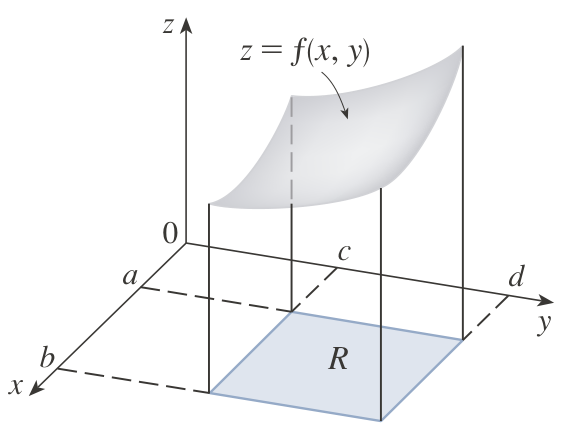
\includegraphics[width=0.5\linewidth]{imagenes/vol-integrado-1.png}
  \caption{Imagen sacada de \parencite{stewart2}. Superficie $ z=f(x,y) $ sobre el rectángulo $ R $.}
  \label{fig:integrales-1}
\end{figure}

Como dijimos, la idea para resolver este cálculo es el mismo que se usa cuando teníamos integrales simples. Lo que vamos a hacer ahora es dividir el rectángulo $ R $ en cuadraditos mas chicos. Esto se hace dividiendo el intervalo $ \left[a,b\right] $ en $ m $ subintervalos $ \left[x_{i-1},x_{i}\right] $ de igual ancho $ \Delta x=(b-a)/m $ y dividiendo $ \left[c,d\right] $ en $ n $ subintervalos $ \left[y_{j-1},y_{j}\right] $ de igual ancho $ \Delta y=(d-c)/n $. Sabemos que cada cuadradito que nos quede tendrá un área determinada, y si multiplicamos ese área por el valor en $ z $ que está asociado al mismo, tenemos el volúmen que hay entre cada cuadradito y la función $ z=f(x,y) $. Esto lo repetimos para todos los cuadrados que tengamos y vamos a tener una aproximación del volúmen de $ S $. 
\[
  V\approx \sum_{i=1}^{m} \sum_{j=1}^{n} f(x_{ij},y_{ij}\Delta A  
\]

Esta doble sumatoria quiere decir que para cada $ i $ se hace la sumatoria desde $ j=1 $ hasta $ j=n $ del producto de $ f(x,y)\cdot \Delta A $. En este caso, la sumatoria de $ j=1 $ se repite $ m $ veces; una para cada $ i $.

\begin{figure}[H]
  \centering
  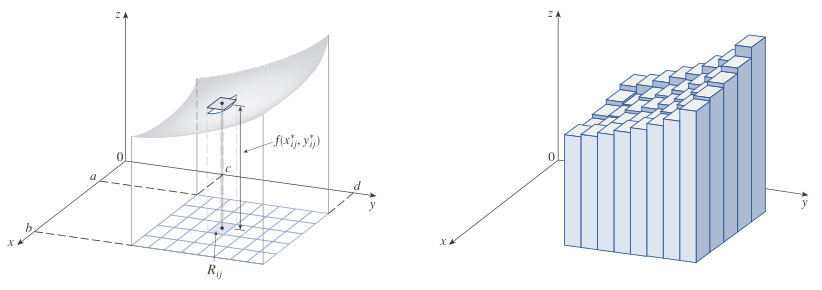
\includegraphics[width=\linewidth]{imagenes/vol-integrado-2.png}
  \caption{Imagen sacada de \parencite{stewart2}. Visualización de la suma doble de Riemann.}
  \label{fig:integrales-2}
\end{figure}

A medida que los cuadrados seán mas y mas chicos, y haya mas y mas cuadrados nos vamos a ir acercando cada vez mas al valor real del volumen. Para lograr esto podemos calcular la suma cuando $ m $ y $ n $ se tienden a infinito, y esto es la definición de una integral doble.

\vspace{0.2cm}
\fbox{\parbox{0.9\linewidth}{
\textbf{Integral doble}

La \textbf{integral doble} de $ f $ en el rectángulo $ R $ es 
\[
  \iint_{R} f(x,y) \,dA = \lim_{m,n \to \infty} f(x_{ij},y_{ij})\Delta A
\]
}}\vspace{0.2cm}

\subsubsection{Integrales iteradas}
Todo esto está muy lindo, pero es muy dificil evaluar las integrales a partir de su definición (mucho mas las integrales dobles). Lo bueno es que las integrales dobles las podemos expresar como integrales iteradas, que después las podemos evaluar como integrales simples.

Supongamos que $ f $ es una función de dos variables integrable en el rectángulo $ R=\left[a,b\right]\times \left[c,d\right] $. Lo que podemos hacer es algo parecido a lo que hacíamos con las derivadas parciales: integramos respecto de alguna variable, digamos $ y $ desde $ c $ hasta $ d $. De esta manera, $ \int_{c}^{d} f(x,y) \,dy $ es un número que depende de $ x $ (ya que acabamos de integrar la variable $ y $), así que la podemos pensar como una función de $ x $:
\[
  H(x)=\int_{c}^{d} f(x,y) \,dy
\]

Y ahora podemos integrar a la función $ H(x) $ desde $ a $ hasta $ b $ como si fuese una integral simple (de hecho, \textbf{es} una integral simple ahora):
\[
  \int_{a}^{b} H(x) \,dx
\]

Como sabemos que $ H(x) $ es la integral de $ f(x,y) $ respecto de $ y $, podemos pensar a la integral doble de la siguiente manera:
\[
  \int_{a}^{b} H(x) \,dx = \int_{a}^{b} \left[\int_{c}^{d} f(x,y) \,dy\right] \,dx = \int_{a}^{b} \int_{c}^{d} f(x,y) \,dy\,dx
\]

\underline{Ejemplo:} Evalar la siguiente integral:
\[
  \int_{0}^{3} \int_{1}^{2} x^2y \,dy\,dx
\]

Por la notación que nos dieron, sabemos que primero tenemos que integrar en $ y $, y el resultado que obtenemos lo integramos en $ x $.

\[
  \int_{1}^{2} x^2y \,dy = \Bigg.x^2\frac{y^2}{2}\Bigg]_{1}^{2} = x^2\left(\frac{4}{2}\right) - x^2\left(\frac{1}{2}\right) = \frac{3}{2}x^2
\]

Ahora tenemos que integrar el resultado obtenido respecto de $ x $
\[
  \int_{0}^{3} \frac{3}{2}x^2 \,dx = \Bigg.\frac{x^3}{2}\Bigg]_{0}^{3}=\frac{27}{2}
\]

\vspace{0.2cm}
\fbox{\parbox{0.9\linewidth}{
\textbf{Teorema de Fubini}

Si $ f $ es continua en el rectángulo $ R=\left\{(x,y) \;/\; a\leq x\leq b \land c\leq y\leq d\right\} $, entonces
\[
  \iint_{R} f(x,y) \,dA = \int_{a}^{b} \int_{c}^{d} f(x,y) \,dy\,dx = \int_{c}^{d} \int_{a}^{b} f(x,y) \,dx\,dy
\]
}}\vspace{0.2cm}

\underline{Ejemplo:} Podemos calcular la integral del ejemplo anterior pero ahora integrando al revés ya que $ f(x,y)=x^2y $ es continua.

Ahora primero intgramos respecto de $ x $.
\[
  \int_{0}^{3} x^2y \,dx = \Bigg.\frac{x^3}{3}y\Bigg]_{0}^{3} = 9
\]

Y luego integramos el resultado de la operación respecto de $ y $.
\[
  \int_{1}^{2} 9y \,dy = \Bigg.\frac{9}{2}y^2\Bigg]_{1}^{2} = 18 - \frac{9}{2} = \frac{27}{2}
\]

Vemos que llegamos al mismo resultado a pesar de haber integrado en distinto orden. Esto solo pasa cuando se cumplen las condiciones del teorema de Fubini.

\underline{Ejemplo de ejercicio de integrales:} Determinar el volumen del sólido $ S $ acotado por el paraboloide elíptico $ x^2+2y^2+z=16 $, los planos $ x=2 $ y $ y=2 $, y los tres planos coordenados.

Lo primero que tenemos que hacer es determinar cuál es la integral que nos pide la consigna que calculemos, y sobre qué región quiere que la calculemos. La consigna habla de un sólido, habíamos visto al principio de esta sección que a la integral doble la podíamos pensar como el volumen del sólido $ S $, estando el sólido por debajo de la función $ z = f(x,y) $ y por encima del rectángulo $ R $.

En este caso la función $ z=f(x,y) $ la despejamos de la ecuación del paraboloide elíptico: $ z = 16-x^2-y^2 $, y el cuadrado $ R $ está dado por los puntos de intersección de los planos coordenados con los planos $ x=2 $ y $ y=2 $. De esta manera, $ R=\left[0,2\right]\times \left[0,2\right] $.
\begin{align*}
  V &= \iint_{R} 16-x^2-y^2 \,dA = \int_{0}^{2} \int_{0}^{2} 16-x^2-y^2 \,dx\,dy\\
   &= \int_{0}^{2} \Bigg.16x-\frac{1}{3}x^3-2y^2x\Bigg]_{x=0}^{x=2} \,dy\\
   &= \int_{0}^{2} \frac{88}{3}-4y^2 \,dy = \Bigg.\frac{88}{3}y-\frac{4}{3}y^3\Bigg]_{0}^{2}=48
\end{align*}

En el caso especial en que $ f(x,y) $ pueda escribirse como el producto de una función que dependa solo de $ x $ y otra que dependa solo de $ y $, podemos escribir la integral doble de una forma mas simple de leer gracias al teorema de Fubini.

Supongamos que tenemos la función $ f(x,y) $ y que la podemos reescribir como $ f(x,y)=g(x)\cdot h(y) $. Entonces:
\[
  \iint_{R} f(x,y) \,dA = \int_{c}^{d} \int_{a}^{b} g(x)\cdot h(y) \,dx\,dy = \int_{c}^{d} \left[\int_{a}^{b} g(x)\cdot h(y) \,dx\right] \,dy
\]

Pero cuando integramos respecto de $ x $, $ y $ es una constante así que la podemos sacar afuera de la integral
\[
  \int_{c}^{d} \left[\int_{a}^{b} g(x)\cdot h(y) \,dx\right] \,dy = \int_{c}^{d} \left[h(y)\cdot \left(\int_{a}^{b} g(x) \,dx\right)\right] \,dy = \int_{a}^{b} g(x) \,dx\cdot \int_{c}^{d} h(y) \,dy
\]

\subsubsection{Valor promedio}
El valor promedio de una función $ f $ de una variable en un intervalo $ \left[a,b\right] $ lo podemos calcular como
\[
  f_{prom}=\frac{1}{b-a}\int_{a}^{b} f(x) \,dx
\]
y tiene sentido. Si queremos calcular el promedio de algo, por ejemplo la nota promedio en una clase, lo que hacemos es sumar las notas de todos los trabajos que había que entregar, y dividimos esa suma por la cantidad de trabajos. Esta fórmula hace lo mismo: la integral suma los resultados de los infinitos puntos en el intervalo $ \left[a,b\right] $ y luego divide ese resultado por el intervalo $ \left[a,b\right] $.

Para funciones de dos variables, el \textbf{valor promedio} se define de forma similar
\[
  f_{prom}=\frac{1}{A(R)}\iint_{R} f(x,y) \,dA
\]
donde $ A(R) $ es el área de R.

\subsection{Integrales dobles en regiones generales}
Ya aprendimos a integrar funciones dentro de regiones cuadradas. Pero la idea es que podamos integrar regiones $ D $ que sean de cualquier forma. Para encontrar una forma de lograr esto vamos a usar un par de truquitos, junto con el teorema de Fubini. 

Si nos piden integrar $ f $ dentro de una región $ D $ que no es un rectángulo, lo primero que vamos a hacer es usar un rectángulo ;) (estos pasos que vienen ahora son simplemente para poder ver de dónde sale la fórmula que nos interesa, no los vamos a volver a usar probablemente). Lo primero que hacemos es armar un rectángulo $ R $ que encierre a la región $ D $ y definimos una nueva función $ F(x,y) $ con dominio $ R $ de la siguiente forma:
\[
  F(x,y)=
  \begin{cases}
  f(x,y) & \text{si (x,y) está en $ D $}\\
  0 & \text{si (x,y) está en $ R $ pero no en $ D $}
  \end{cases}
\]

\begin{figure}[H]
  \centering
  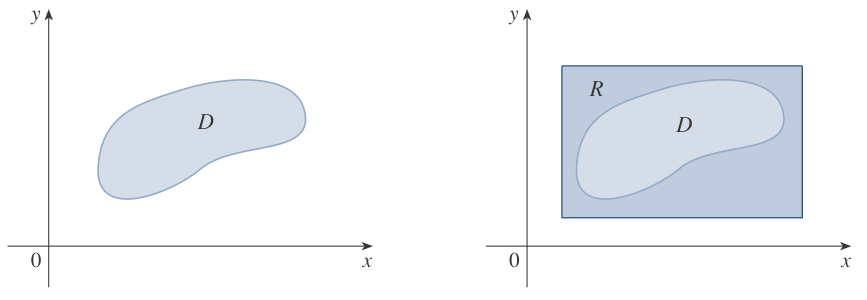
\includegraphics[width=\linewidth]{imagenes/integral-region-general.png}
  \caption{Imagen sacada de \parencite{stewart2}. Visualización de la región $ R $ que contiene a $ D $.}
  \label{fig:integral-region-general}
\end{figure}

Se dice que una región $ D $ en un plano es de \textbf{tipo I} si la podemos definir entre las gráficas de dos funciones continuas de $ x $, es decir
\[
  D=\left\{(x,y)  \;/\;  a\leq x\leq b, g_{1}(x)\leq y\leq g_{2}(x)\right\}
\]
donde $ g_{1} $ y $ g_{2} $ son continuas en $ \left[a,b\right] $. En la figura \ref{fig:regiones-tipo-1} se ven algunos ejemplos de estas regiones.

\begin{figure}[H]
  \centering
  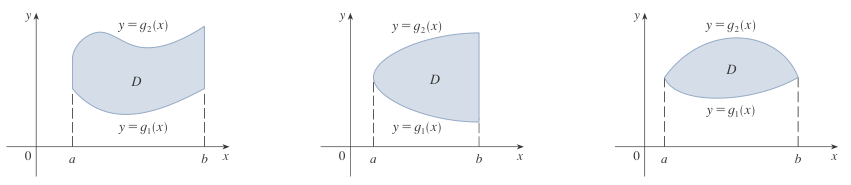
\includegraphics[width=\linewidth]{imagenes/regiones-tipo-1.png}
  \caption{Imagen sacada de \parencite{stewart2}. Algunas regiones tipo I.}
  \label{fig:regiones-tipo-1}
\end{figure}

Para evaluar $ \iint_{D} f(x,y) \,dA $ cuando $ D $ es una región de tipo I, elegimos un rectángulo $ R=\left[a,b\right]\times \left[c,d\right] $ que contenga $ D $, y definimos $ F $ como dijimos mas arriba. Así, por el teorema de Fubini,
\[
  \iint_{D} f(x,y) \,dA=\iint_{R} F(x,y) \,dA=\int_{a}^{b} \int_{c}^{d} F(x,y) \,dy\,dx
\]

Al estar en una región de tipo I, y por cómo está definida $ F $ sabemos que $ F(x,y)=0 $ si $ y<g_{1}(x) $ o $ y>g_{2}(x) $. Por lo tanto,
\[
  \int_{c}^{d} F(x,y) \,dy = \int_{g_{1}(x)}^{g_{2}(x)} F(x,y) \,dy=\int_{g_{1}(x)}^{g_{2}(x)} f(x,y) \,dy
\]
porque $ F(x,y)=f(x,y) $ cuando $ g_{1}(x)\leq y\leq g_{2}(x) $.

\vspace{0.2cm}
\fbox{\parbox{0.9\linewidth}{
\textbf{}

Si $ f $ es continua en una región $ D $ tipo I, tal que 
\[
  D=\left\{(x,y) \;/\; a\leq x\leq b \land g_{1}(x)\leq y\leq g_{2}(x)\right\}
\]
entonces
\[
  \iint_{D} f(x,y) \,dA = \int_{a}^{b} \int_{g_{1}(x)}^{g_{2}(x)} f(x,y) \,dy\,dx
\]
}}\vspace{0.2cm}

También existen las regiones en un plano de \textbf{tipo II}, que pueden expresarse como
\[
  D=\left\{(x,y) \;/\; c\leq y\leq d \land h_{1}(y)\leq x\leq h_{2}(y)\right\}
\]
donde $ h_{1} $ y $ h_{2} $ son continuas.

Usando los mismo métodos que usamos recién, podemos demostrar que

\vspace{0.2cm}
\fbox{\parbox{0.9\linewidth}{
\textbf{}
\[
  \iint_{D} f(x,y) \,dA=\int_{c}^{d} \int_{h_{1}(y)}^{h_{2}(y)} f(x,y) \,dx\,dy
\]
donde $ D $ es una región de tipo II.
}}\vspace{0.2cm}

\underline{Ejemplo 1:} Evluar $ \iint_{D} x+2y \,dA $, donde $ D $ es la región acotada por las parábolas $ y=2x^2 $ y $ y=1+x^2 $.

\begin{figure}[htbp]
  \centering
  {\large }
  \tikzsetnextfilename{regiones-1}
  \begin{tikzpicture}
    \begin{axis}[
      clip=false,
      xlabel={$x$}, ylabel={$y$},
      axis lines=center,
      axis on top=true,
      width=10cm,
    ]
      \addplot [black, thick, name path=A, domain=-1.2:1.2] {2*x^2}
          node[right, pos=0.60] {$ y=2x^2 $};
      \addplot [black, thick, name path=B, domain=-1.2:1.2,] {1+x^2}
	  node[above, pos=0.60, yshift=10pt] {$ y=1+x^2 $};
      \addplot [blue!30] fill between [of=A and B, soft clip={domain=-1:1}];
    \end{axis}
  \end{tikzpicture}
  \caption{Ejemplo 1}
  \label{grf:regiones1}
\end{figure}


\newpage
\addcontentsline{toc}{section}{Referencias}
\printbibliography

\end{document}
